\documentclass[11pt,a4paper]{article}
\usepackage[margin=2.3cm]{geometry}
\usepackage[utf8]{inputenc}
\usepackage{amsmath,amssymb,amsthm,mathtools,bm}
\usepackage{microtype,booktabs,enumitem,xcolor,array}
\usepackage[most]{tcolorbox}
\usepackage{tikz}
\usetikzlibrary{arrows.meta,positioning,calc,shapes.geometric,decorations.pathreplacing,fit,backgrounds}
\usepackage{pgfplots}
\pgfplotsset{compat=1.17}
\pgfplotsset{every axis/.append style={font=\small, tick label style={font=\footnotesize}, label style={font=\small}, legend style={font=\footnotesize}}}
\usepackage[hidelinks]{hyperref}
\usepackage{caption}
\captionsetup{font=small,labelfont=bf}
\setlist{itemsep=2pt,topsep=3pt}
\setlength{\parindent}{0pt}
\setlength{\parskip}{5pt}

% ---------- macros ----------
\newcommand{\R}{\mathbb{R}}
\newcommand{\E}{\mathbb{E}}
\newcommand{\cS}{\mathcal{S}}
\newcommand{\cA}{\mathcal{A}}
\newcommand{\Bell}{\mathcal{B}}
\newcommand{\Bpi}{\mathcal{B}^{\pi}}
\newcommand{\norm}[1]{\lVert #1\rVert_\infty}
\newcommand{\abs}[1]{\left\lvert #1\right\rvert}
\DeclareMathOperator*{\argmax}{arg\,max}
\newcommand{\slides}[1]{\texorpdfstring{\emph{(slides #1)}}{(slides #1)}}
\newcommand{\slide}[1]{\texorpdfstring{\emph{(slide #1)}}{(slide #1)}}
\newcommand{\pdfnum}[1]{\setcounter{theorem}{\numexpr #1-1\relax}}

% ---------- theorem-like environments ----------
% Numbers 1--8 and letters A,B follow the companion note L04-1; S/L/E/F items are added from the slides or recalled.
\theoremstyle{plain}
\newtheorem{theorem}{Theorem}
\newtheorem{corollary}[theorem]{Corollary}
\newtheorem{proposition}{Proposition}\renewcommand{\theproposition}{S\arabic{proposition}}
\newtheorem{lemma}{Lemma}\renewcommand{\thelemma}{L\arabic{lemma}}
\theoremstyle{definition}
\newtheorem{definition}[theorem]{Definition}
\newtheorem{example}{Example}\renewcommand{\theexample}{E\arabic{example}}
\newtheorem{algorithm}{Algorithm}\renewcommand{\thealgorithm}{\Alph{algorithm}}
\newtheorem{fact}{Fact}\renewcommand{\thefact}{F\arabic{fact}}
\theoremstyle{remark}
\newtheorem*{remark}{Remark}

\tcbset{thmbase/.style={enhanced, breakable, sharp corners, boxrule=0.5pt, left=6pt, right=6pt, top=3pt, bottom=3pt, before skip=9pt, after skip=9pt}}
\tcolorboxenvironment{theorem}{thmbase, colback=red!4!white, colframe=red!55!black}
\tcolorboxenvironment{corollary}{thmbase, colback=red!4!white, colframe=red!55!black}
\tcolorboxenvironment{proposition}{thmbase, colback=orange!6!white, colframe=orange!70!black}
\tcolorboxenvironment{lemma}{thmbase, colback=orange!6!white, colframe=orange!70!black}
\tcolorboxenvironment{definition}{thmbase, colback=green!5!white, colframe=green!45!black}
\tcolorboxenvironment{example}{thmbase, colback=teal!5!white, colframe=teal!60!black}
\tcolorboxenvironment{algorithm}{thmbase, colback=violet!5!white, colframe=violet!60!black}
\tcolorboxenvironment{fact}{thmbase, colback=black!4!white, colframe=black!50}

\newtcolorbox{intuition}{enhanced, breakable, colback=blue!6!white, colframe=blue!60!black, boxrule=0.5pt,
  coltitle=white, fonttitle=\bfseries\small, title={Intuition}, left=6pt, right=6pt, top=3pt, bottom=3pt,
  attach boxed title to top left={yshift=-2mm, xshift=3mm}, boxed title style={colback=blue!60!black, sharp corners},
  before skip=14pt, after skip=9pt}

\newcommand{\figref}[1]{Figure~\ref{#1}}

% TikZ styles
\tikzset{
  box/.style={draw, rounded corners=2pt, minimum height=8mm, minimum width=18mm, align=center, fill=white},
  st/.style={circle, draw, minimum size=8mm, inner sep=1pt, fill=green!12},
  act/.style={circle, fill=black, inner sep=1.3pt},
  >=Stealth
}

\title{\textbf{Value Iteration}\\[2pt]\large Lecture Notes --- Reinforcement Learning 2026--27, Deck L04}
\author{Based on slides L04 (slides 1--75) and the companion note \texttt{L04-1-value-iteration.pdf}}
\date{}

\begin{document}
\maketitle

\begin{abstract}\noindent
This lecture answers the question left open by the MDP lectures: \emph{how do we actually compute} $V^\pi$ and, above all, the optimal policy $\pi^*$?
We first compute $V^\pi$ exactly (a linear system) and iteratively (a fixed-point iteration), introduce \emph{contraction mappings} as the tool that makes iteration converge, show that both Bellman backups are $\gamma$-contractions, and conclude with \textbf{value iteration}, its convergence rate, the quality of the greedy policy it returns, and the number of iterations needed for an $\epsilon$-optimal policy.
\end{abstract}

\subsection*{How these notes are organised}
\begin{itemize}
  \item \textbf{Sections follow the slide deck}, with the slide range in italics next to each title. Formal material from the companion note is merged where the slides introduce the topic.
  \item \textbf{Numbering.} Definitions, theorems and corollaries \emph{1--8} and algorithms \emph{A, B} keep the numbering of the companion note, so that its self-check list and proof videos map directly (see Appendix~\ref{app:selfcheck}). Items numbered \emph{S, L, E, F} are not in the companion note: \emph{S}/\emph{L} = propositions/lemmas derived on the slides (or needed for completeness), \emph{E} = worked examples, \emph{F} = facts recalled from the previous lecture (L03).
  \item \textbf{Coloured boxes.} Definitions (green), theorems/corollaries (red), propositions/lemmas (orange), examples (teal), algorithms (violet), recalled facts (grey), and blue \emph{Intuition} boxes that explain the ``why'' in plain words.
  \item \textbf{Running example.} A tiny two-state, two-action MDP (Example~\ref{ex:toy}) is used for all worked numbers and for the data-driven plots.
  \item \textbf{Supplementary material} not covered on the slides (the existence/rate part of Banach's theorem) is in Appendix~\ref{app:banach}, clearly labelled.
\end{itemize}
Throughout, rewards lie in $[0,1]$ (so $R_{\max}=1$), $\gamma\in[0,1)$, $\norm{\cdot}$ is the sup-norm, and $\ln$ is the natural logarithm (the slides write $\log$ for it).

\tableofcontents
\newpage
%=====================================================================
\section{Recap: Sequential Decision Making and MDPs \slides{2--12}}
%=====================================================================
This block repeats what the previous lecture (L03) established. Everything later is built on it, and three of the results are quoted from L03 without proof (Facts F1--F4 below).

\subsection{Sequential Decision Making and the MDP \slides{3--4}}
The agent interacts with its environment at discrete timesteps: at each step it receives an observation $o_t$ and a reward $r_t$ from the environment and answers with an action $a_t$ (\figref{fig:loop}). The \emph{state} is a function of the history, $s_t=f(h_t)$, and is typically hidden or unknown.

A \textbf{Markov Decision Process} is sequential decision making under the Markov assumption: the transition dynamics are Markovian, the state is fully observable, and the dynamics are (in general) stochastic, $p(s_{t+1}\mid s_t,a_t)$. Equivalent shorthand: $s_{t+1}\sim p(\cdot\mid s_t,a_t)$ or $s'\sim p(\cdot\mid s,a)$. An MDP is the tuple $(\cS,\cA,p,r,\gamma)$ with set of states $\cS$, set of actions $\cA$, transition kernel $p$, reward $r(s,a)$ and discount $\gamma$.

\begin{figure}[htbp]
\centering
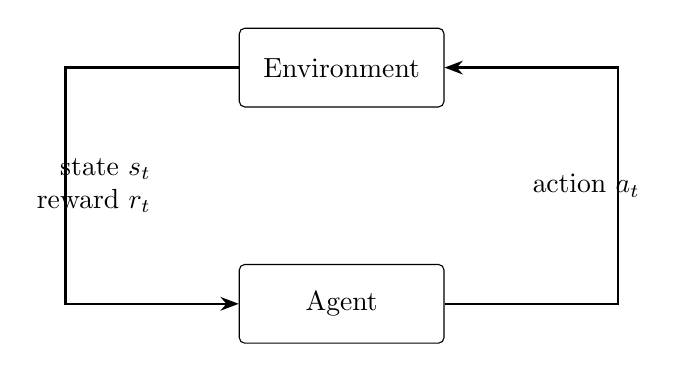
\begin{tikzpicture}
  \node[box, minimum width=26mm, minimum height=10mm] (agent) at (0,0) {Agent};
  \node[box, minimum width=26mm, minimum height=10mm] (env) at (0,3) {Environment};
  \draw[->, thick] (agent.east) -- ++(2.2,0) |- (env.east);
  \draw[->, thick] (env.west) -- ++(-2.2,0) |- (agent.west);
  \node[right] at (2.3,1.5) {action $a_t$};
  \node[left, align=right] at (-2.3,1.5) {state $s_t$\\ reward $r_t$};
\end{tikzpicture}
\caption{The agent--environment loop (redrawn from slides 3--4). The environment answers each action with a new state/observation and a reward.}
\label{fig:loop}
\end{figure}

\begin{intuition}
The Markov property says that \emph{the present state is a sufficient summary of the past}: once you know $s_t$ and $a_t$, the history tells you nothing more about where you will go next. That is why a policy can be a function of the current state alone, and why value functions can be defined state by state.
\end{intuition}

\subsection{Policies, Value Functions and Q-Functions \slides{5--6}}
A \textbf{policy} $\pi$ is a mapping from (all) states to actions; it determines how the agent selects actions. It can be \emph{deterministic}, $a=\pi(s)$, or \emph{stochastic}, $\pi(a\mid s)$ (also written $p(a\mid s)$ or $a\sim\pi(\cdot\mid s)$).

The \textbf{value function} and \textbf{Q-function} of $\pi$ measure how good states and actions are, and give a way to compare policies:
\[
V^\pi(s)=\E_\pi\Big[\sum_{h\ge0}\gamma^h r_{t+h}\;\Big|\;s_t=s\Big],\qquad
Q^\pi(s,a)=\E_\pi\Big[\sum_{h\ge0}\gamma^h r_{t+h}\;\Big|\;s_t=s,\,a_t=a\Big],
\]
where after the first step actions follow $\pi$ and next states are drawn from $p$. For infinite-horizon MDPs there always exists a \emph{deterministic} policy $\pi^*$ with $V^{\pi^*}(s)\ge V^\pi(s)$ for all $s$ and all $\pi$: the optimal policy \emph{dominates every other policy in every state}. We write $V^*=V^{\pi^*}$ and $Q^*=Q^{\pi^*}$.

\begin{intuition}
Comparing two policies means comparing two vectors $V^\pi,V^{\pi'}\in\R^{|\cS|}$, which is only a \emph{partial} order: $\pi$ might be better in one state and worse in another. The nontrivial fact is that for discounted infinite-horizon MDPs a single deterministic $\pi^*$ is best \emph{in every state at once}, so ``find the optimal policy'' is a well-posed goal.
\end{intuition}

\subsection{The Discount Factor \slide{7}}
Setting $\gamma=1$ for infinite tasks is a bad idea: the sum of rewards may diverge. For $\gamma\in[0,1)$ the weights form a geometric series,
\[
\sum_{h=0}^{\infty}\gamma^h=\frac1{1-\gamma},
\]
so the value of $\gamma$ roughly determines \emph{how many steps ahead we are looking}: $\gamma=0.99$ corresponds to a horizon of about $100$ steps (the slide rounds this to ``99 timesteps ahead''). This also bounds all values:

\begin{fact}[L03-1, Lemma 3 --- range of values]\label{fact:range}
If $r(s,a)\in[0,R_{\max}]$ then $0\le V^\pi(s),V^*(s),Q^\pi(s,a),Q^*(s,a)\le R_{\max}/(1-\gamma)$. (Each is a discounted sum of terms in $[0,R_{\max}]$, bounded by $R_{\max}\sum_h\gamma^h$.) With $R_{\max}=1$ this is the interval $[0,1/(1-\gamma)]$ used on the slides.
\end{fact}

\begin{figure}[htbp]
\centering
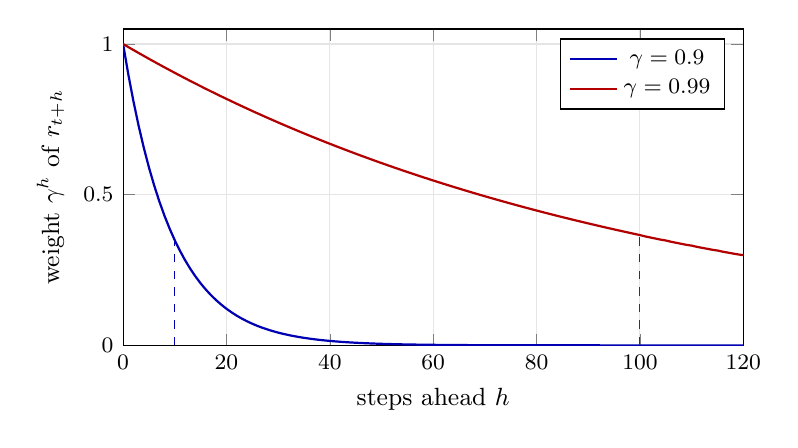
\begin{tikzpicture}
\begin{axis}[width=0.78\linewidth, height=5.6cm, xmin=0, xmax=120, ymin=0, ymax=1.05, xlabel={steps ahead $h$}, ylabel={weight $\gamma^h$ of $r_{t+h}$},
  legend pos=north east, grid=both, grid style={gray!20}]
\addplot[blue!70!black, thick, domain=0:120, samples=121] {0.9^x};
\addplot[red!70!black, thick, domain=0:120, samples=121] {0.99^x};
\addplot[blue!70!black, dashed] coordinates {(10,0)(10,0.349)};
\addplot[red!70!black, dashed] coordinates {(100,0)(100,0.366)};
\legend{$\gamma=0.9$, $\gamma=0.99$}
\end{axis}
\end{tikzpicture}
\caption{Weight of the reward received $h$ steps ahead (original figure; slide 7 only describes this in prose). Dashed lines mark the effective horizon $1/(1-\gamma)$, where the weight has dropped to about $e^{-1}\approx0.37$.}
\label{fig:discount}
\end{figure}

\begin{intuition}
Think of $\gamma$ as a ``patience'' dial. With $\gamma=0.9$ rewards more than $\sim10$ steps away barely matter; with $\gamma=0.99$ the agent looks $\sim100$ steps ahead. The same number $1/(1-\gamma)$ reappears in this lecture as (i) the largest possible value, (ii) the initialisation range for the iterations, and (iii) the factor that inflates the error of the greedy policy. Larger $\gamma$ means a longer horizon and harder computation.
\end{intuition}

\subsection{Bellman Expectation Equation \slide{8}}
The value of a state is expanded in terms of the current reward and the value of the next states, according to the policy:
\begin{align*}
V^\pi(s)&=r(s,\pi(s))+\gamma\,\E_{s'\sim p(\cdot\mid s,\pi(s))}\big[V^\pi(s')\big],\\
Q^\pi(s,a)&=r(s,a)+\gamma\,\E_{s'\sim p(\cdot\mid s,a)}\big[V^\pi(s')\big],\qquad V^\pi(s)=Q^\pi(s,\pi(s)).
\end{align*}
In the first line the reward is a function of $s$ and $\pi(s)$; in the second, of $s$ and $a$.

\begin{fact}[L03-1, Theorem 6 --- Bellman expectation equation]\label{fact:bexp}
For every policy $\pi$ and every state $s$, the display above holds. In operator language (Definition~\ref{def:bellman}): $\Bpi V^\pi=V^\pi$.
\end{fact}

\begin{intuition}
A one-step lookahead: \emph{what you get now} plus \emph{the discounted value of wherever you land}, averaged over the randomness of the transition. It turns an infinite sum into a \emph{local} consistency condition that must hold in all states simultaneously, and that is exactly what we will exploit to compute $V^\pi$.
\end{intuition}

\subsection{Bellman Optimality \slides{9--12}}
\textbf{Example (slide 9).} Suppose we already know $V^*$ at the successor states $s'$ and $s''$. From $s$ we try each action: taking $a'$ gives reward $r(s,a')$ and leads to $s'$, so $Q^*(s,a')=r(s,a')+\gamma V^*(s')$; likewise $Q^*(s,a'')=r(s,a'')+\gamma V^*(s'')$. Then $V^*(s)=\max\{Q^*(s,a'),Q^*(s,a'')\}$ (\figref{fig:tree}; the slide draws deterministic transitions, with stochastic ones $V^*(s')$ becomes an expectation).

\begin{figure}[htbp]
\centering
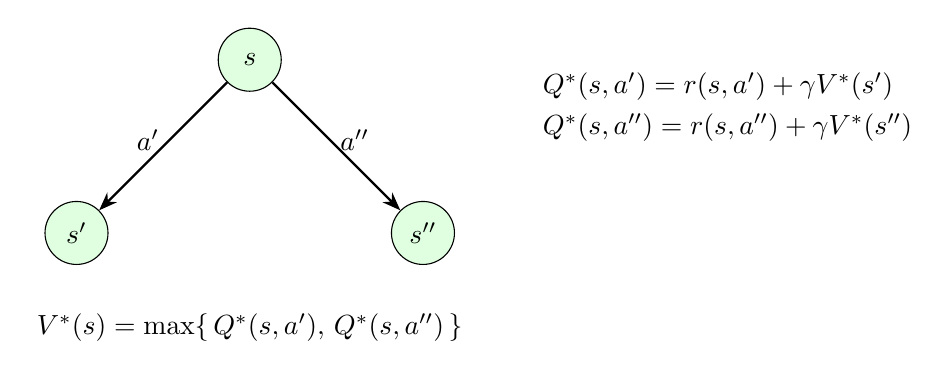
\begin{tikzpicture}
  \node[st] (s) at (0,0) {$s$};
  \node[st] (s1) at (-2.2,-2.2) {$s'$};
  \node[st] (s2) at (2.2,-2.2) {$s''$};
  \draw[->, thick] (s) -- node[left, pos=0.45] {$a'$} (s1);
  \draw[->, thick] (s) -- node[right, pos=0.45] {$a''$} (s2);
  \node[align=left, anchor=west] at (3.6,-0.6) {$Q^*(s,a')=r(s,a')+\gamma V^*(s')$\\[3pt] $Q^*(s,a'')=r(s,a'')+\gamma V^*(s'')$};
  \node at (0,-3.4) {$V^*(s)=\max\{\,Q^*(s,a'),\,Q^*(s,a'')\,\}$};
\end{tikzpicture}
\caption{Bellman optimality backup in one picture (redrawn from slide 9): try every action, evaluate it with the (assumed known) values of the successors, keep the best.}
\label{fig:tree}
\end{figure}

In general,
\[
V^*(s)=\max_a\Big[r(s,a)+\gamma\,\E_{s'\sim p(\cdot\mid s,a)}V^*(s')\Big],\qquad
Q^*(s,a)=r(s,a)+\gamma\,\E_{s'\sim p(\cdot\mid s,a)}\Big[\max_{a'}Q^*(s',a')\Big].
\]
Two results from L03 are quoted on the slides:

\begin{fact}[Slide 10 ``Theorem 1'', L03-1 Theorem 8 --- Bellman optimality]\label{fact:bopt}
$V^*$ and $Q^*$ satisfy the two equations above, and the greedy policy $\hat\pi(s)\in\argmax_aQ^*(s,a)$ satisfies $V^{\hat\pi}=V^*$. Hence $\pi^*(s)=\argmax_aQ^*(s,a)$ is an optimal policy.
\end{fact}

\begin{fact}[Slide 11 ``Theorem 2'', L03-1 Theorem 10 --- uniqueness]\label{fact:uniq}
For any $V$, if $V(s)=\max_a\big[r(s,a)+\gamma\E_{s'\sim p(\cdot\mid s,a)}V(s')\big]$ for all $s$, then $V=V^*$.
\end{fact}

\begin{intuition}
The optimality equation lets us \emph{focus on one step at a time}: we only choose the best first action and leave the rest of the problem to $V(s')$. Fact~\ref{fact:uniq} says that any function that is locally self-consistent in this sense \emph{is} $V^*$: there is nothing else to look for. Fact~\ref{fact:bopt} converts $Q^*$ into a policy by a plain $\argmax$. Together they say: \emph{find the unique solution of the Bellman optimality equation and you are done}. How to find it is the subject of the rest of the lecture. (The proof of uniqueness in L03 was a long unrolling argument; Corollary~\ref{cor:fixed} below re-proves it in one line.) \slide{12} closes the recap.
\end{intuition}
%=====================================================================
\section{Policy Evaluation \slides{13--15}}
%=====================================================================
\textbf{Question.} Given an MDP $(\cS,\cA,p,r,\gamma)$ and a policy $\pi$, how can we compute the goodness of $\pi$, i.e.\ $V^\pi$?

\textbf{Why is this interesting?} There are $|\cA|^{|\cS|}$ possible deterministic policies, and we want to find the optimal one. To find it, we need to be able to \emph{evaluate} candidates.

\begin{intuition}
Policy evaluation is the ``scoring function'' of reinforcement learning: before you can say that one policy is better than another you need a number (really, a vector with one entry per state) that says how well each one does. Everything in this lecture is about computing such numbers cheaply: first for a \emph{given} policy, then for the \emph{best} policy at once.
\end{intuition}

%=====================================================================
\section{Exact Policy Evaluation \slides{16--22}}\label{sec:exact}
%=====================================================================
\emph{Note: the companion note marks this block as ``on the slides only'': it is not proved there, so prepare it from the slides.}

Given $(\cS,\cA,p,r,\gamma)$ and $\pi$, what is $V^\pi$? We know that the Bellman expectation equation holds for \emph{all} states:
\[
V^\pi(s)=r(s,\pi(s))+\gamma\sum_{s'\in\cS}p(s'\mid s,\pi(s))\,V^\pi(s').
\]
\emph{How many linear constraints do we have?} $|\cS|$, one per state, in the $|\cS|$ unknowns $V^\pi(s)$. We can combine all the constraints (slide credit: Wen Sun). Define the reward vector and the transition matrix induced by $\pi$:
\[
r^\pi\in\R^{|\cS|},\ (r^\pi)_s=r(s,\pi(s));\qquad
P^\pi\in\R^{|\cS|\times|\cS|},\ (P^\pi)_{s,s'}=p(s'\mid s,\pi(s)).
\]
Then the $|\cS|$ equations read $V^\pi=r^\pi+\gamma P^\pi V^\pi$ (\figref{fig:matrix}), which we can solve for $V^\pi$.

\begin{figure}[htbp]
\centering
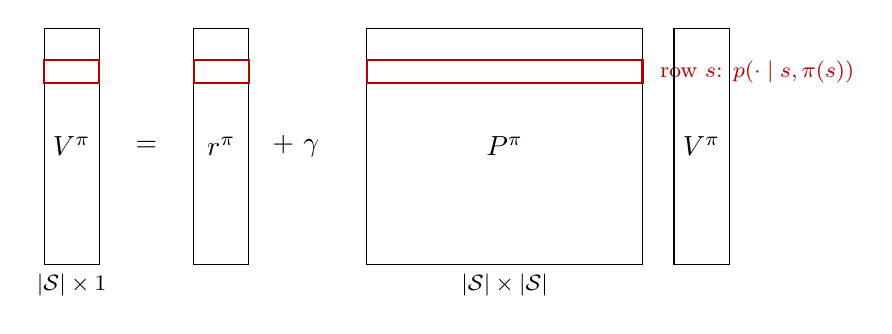
\begin{tikzpicture}[x=1cm,y=1cm]
  % V
  \draw (0,0) rectangle (0.7,3); \node at (0.35,1.5) {$V^\pi$};
  \node at (1.3,1.5) {$=$};
  \draw (1.9,0) rectangle (2.6,3); \node at (2.25,1.5) {$r^\pi$};
  \node at (3.2,1.5) {$+\ \gamma$};
  \draw (4.1,0) rectangle (7.6,3); \node at (5.85,1.5) {$P^\pi$};
  \draw[red!70!black, thick] (4.1,2.3) rectangle (7.6,2.6);
  \node[red!70!black, font=\footnotesize, anchor=west] at (7.7,2.45) {row $s$: $p(\cdot\mid s,\pi(s))$};
  \draw (8.0,0) rectangle (8.7,3); \node at (8.35,1.5) {$V^\pi$};
  \draw[red!70!black, thick] (0,2.3) rectangle (0.7,2.6);
  \draw[red!70!black, thick] (1.9,2.3) rectangle (2.6,2.6);
  \node[font=\footnotesize, below] at (0.35,0) {$|\cS|\times1$};
  \node[font=\footnotesize, below] at (5.85,0) {$|\cS|\times|\cS|$};
\end{tikzpicture}
\caption{The $|\cS|$ Bellman expectation equations stacked in matrix form (redrawn from slides 20--22). The highlighted row is the equation for one state $s$: $V^\pi(s)=r(s,\pi(s))+\gamma\,\langle p(\cdot\mid s,\pi(s)),V^\pi\rangle$.}
\label{fig:matrix}
\end{figure}

\begin{proposition}[Exact policy evaluation, slides 21--22]\label{prop:exact}
For $\gamma<1$, the matrix $I-\gamma P^\pi$ is invertible and
\[
V^\pi=(I-\gamma P^\pi)^{-1}r^\pi=\sum_{k\ge0}\gamma^k(P^\pi)^kr^\pi .
\]
Computing it by matrix inversion costs $O(|\cS|^3)$.
\end{proposition}
\begin{proof}
$P^\pi$ is row-stochastic (entries $\ge0$, each row sums to $1$), so its induced $\infty$-norm is $1$ and $\norm{\gamma P^\pi x}\le\gamma\norm{x}$. If $(I-\gamma P^\pi)x=0$ then $x=\gamma P^\pi x$, so $\norm{x}\le\gamma\norm{x}$, forcing $x=0$ since $\gamma<1$; hence the matrix is invertible. The Neumann series $\sum_k(\gamma P^\pi)^k$ converges (its terms have norm $\le\gamma^k$) and equals the inverse. Rearranging $V^\pi=r^\pi+\gamma P^\pi V^\pi$ gives $(I-\gamma P^\pi)V^\pi=r^\pi$. Inverting an $|\cS|\times|\cS|$ matrix takes $O(|\cS|^3)$ operations.
\end{proof}

\begin{intuition}
The Neumann series is the Bellman equation unrolled: $(P^\pi)^kr^\pi$ is the expected reward $k$ steps ahead, and $\gamma^k$ discounts it, so $V^\pi$ is literally the \emph{expected discounted sum of rewards}. The closed form is ``nice but computationally expensive'' (the slide's own verdict): cubic in the number of states is fine for dozens of states but hopeless for millions. This motivates an approach that only needs matrix--vector products.
\end{intuition}

\begin{example}[A two-state MDP, used throughout]\label{ex:toy}
Take $\cS=\{s_1,s_2\}$, $\cA=\{a,b\}$, $\gamma=0.9$, with
\begin{center}
\begin{tabular}{@{}lccc@{}}
\toprule
$(s,\text{action})$ & $r$ & $p(s_1\mid\cdot)$ & $p(s_2\mid\cdot)$\\
\midrule
$(s_1,a)$ & $0$ & $0.5$ & $0.5$\\
$(s_1,b)$ & $0.5$ & $1$ & $0$\\
$(s_2,a)$ & $1$ & $0.1$ & $0.9$\\
$(s_2,b)$ & $0.2$ & $1$ & $0$\\
\bottomrule
\end{tabular}
\end{center}
\begin{center}
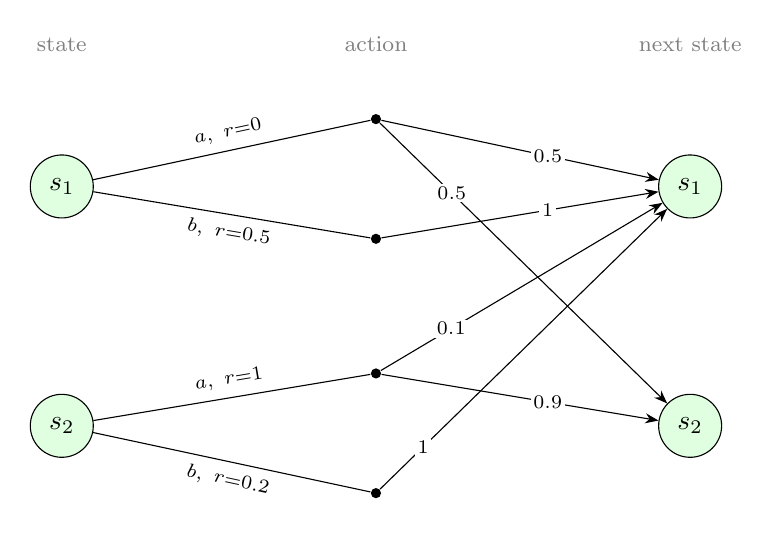
\begin{tikzpicture}[scale=0.95]
  \node[font=\footnotesize, gray] at (0,3.5) {state};
  \node[font=\footnotesize, gray] at (4.2,3.5) {action};
  \node[font=\footnotesize, gray] at (8.4,3.5) {next state};
  \node[st] (s1) at (0,1.6) {$s_1$};
  \node[st] (s2) at (0,-1.6) {$s_2$};
  \node[act] (a1) at (4.2,2.5) {};
  \node[act] (b1) at (4.2,0.9) {};
  \node[act] (a2) at (4.2,-0.9) {};
  \node[act] (b2) at (4.2,-2.5) {};
  \node[st] (t1) at (8.4,1.6) {$s_1$};
  \node[st] (t2) at (8.4,-1.6) {$s_2$};
  \draw (s1) -- node[above, sloped, font=\scriptsize, pos=0.5] {$a,\ r{=}0$} (a1);
  \draw (s1) -- node[below, sloped, font=\scriptsize, pos=0.5] {$b,\ r{=}0.5$} (b1);
  \draw (s2) -- node[above, sloped, font=\scriptsize, pos=0.5] {$a,\ r{=}1$} (a2);
  \draw (s2) -- node[below, sloped, font=\scriptsize, pos=0.5] {$b,\ r{=}0.2$} (b2);
  \draw[->] (a1) -- node[fill=white, inner sep=1pt, font=\scriptsize, pos=0.6] {$0.5$} (t1);
  \draw[->] (a1) -- node[fill=white, inner sep=1pt, font=\scriptsize, pos=0.25] {$0.5$} (t2);
  \draw[->] (b1) -- node[fill=white, inner sep=1pt, font=\scriptsize, pos=0.6] {$1$} (t1);
  \draw[->] (a2) -- node[fill=white, inner sep=1pt, font=\scriptsize, pos=0.25] {$0.1$} (t1);
  \draw[->] (a2) -- node[fill=white, inner sep=1pt, font=\scriptsize, pos=0.6] {$0.9$} (t2);
  \draw[->] (b2) -- node[fill=white, inner sep=1pt, font=\scriptsize, pos=0.15] {$1$} (t1);
\end{tikzpicture}
\end{center}
Filled dots are state-action pairs; the arrows leaving a dot are the stochastic transitions, labelled with their probabilities. For the policy $\pi=(a,a)$ (always play $a$):
\[
P^\pi=\begin{pmatrix}0.5&0.5\\0.1&0.9\end{pmatrix},\quad r^\pi=\begin{pmatrix}0\\1\end{pmatrix},\quad
I-\gamma P^\pi=\begin{pmatrix}0.55&-0.45\\-0.09&0.19\end{pmatrix},\quad \det=0.064,
\]
\[
V^\pi=(I-\gamma P^\pi)^{-1}r^\pi=\frac1{0.064}\begin{pmatrix}0.19&0.45\\0.09&0.55\end{pmatrix}\begin{pmatrix}0\\1\end{pmatrix}
=\begin{pmatrix}7.03125\\8.59375\end{pmatrix}.
\]
It will turn out that this policy is in fact optimal for this MDP: $V^*=(7.03125,\,8.59375)$.
\end{example}

%=====================================================================
\section{Fixed-Point Iteration \slides{23--24}}
%=====================================================================
What is a \textbf{fixed point}? A point $x$ such that $x=f(x)$. How can we find such points?
\begin{enumerate}[label=\arabic*.]
  \item Initialise $x_0$.
  \item Repeat $x_{i+1}=f(x_i)$.
  \item Stop at convergence, when $x$ does not change any more.
\end{enumerate}
Geometrically (slide 24), fixed points are the intersections of $y=f(x)$ with the line $y=x$. The iteration is a ``cobweb'': from $(x_i,x_i)$ on the diagonal go vertically to the curve at $(x_i,x_{i+1})$, then horizontally back to the diagonal at $(x_{i+1},x_{i+1})$. The slide's example is $f(x)=\cos x$, with fixed point $x^*\approx0.739085$.

\begin{figure}[htbp]
\centering
\begin{minipage}{0.52\linewidth}
\centering
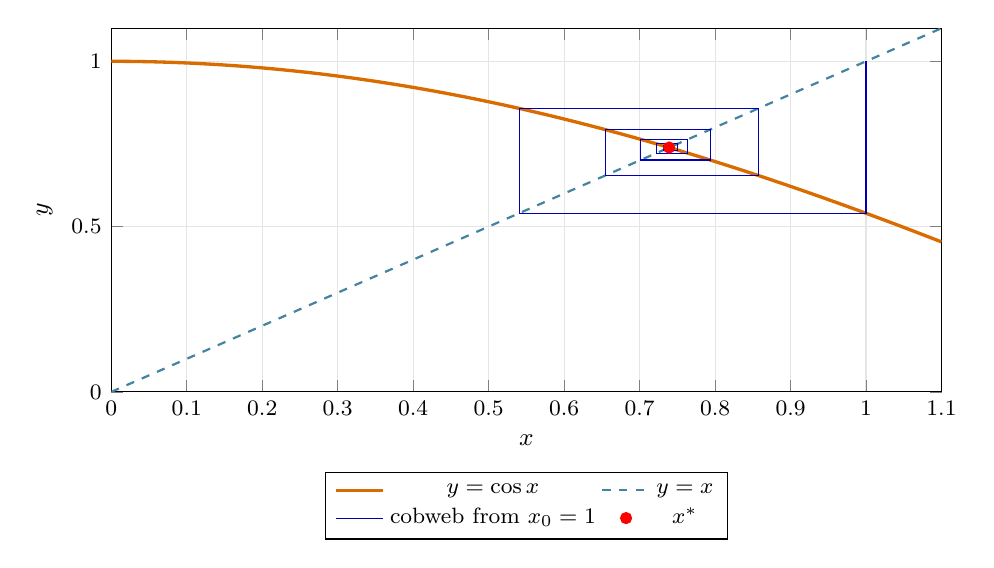
\begin{tikzpicture}
\begin{axis}[width=\linewidth, height=6.2cm, xmin=0, xmax=1.1, ymin=0, ymax=1.1, xlabel={$x$}, ylabel={$y$}, legend style={at={(0.5,-0.22)}, anchor=north, legend columns=2}, grid=both, grid style={gray!20}]
\addplot[orange!85!black, very thick, domain=0:1.1, samples=60] {cos(deg(x))};
\addplot[cyan!60!black, dashed, thick, domain=0:1.1] {x};
\addplot[blue!70!black, thin] coordinates {(1.000000,1.000000) (1.000000,0.540302) (0.540302,0.540302) (0.540302,0.540302) (0.540302,0.857553) (0.857553,0.857553) (0.857553,0.857553) (0.857553,0.654290) (0.654290,0.654290) (0.654290,0.654290) (0.654290,0.793480) (0.793480,0.793480) (0.793480,0.793480) (0.793480,0.701369) (0.701369,0.701369) (0.701369,0.701369) (0.701369,0.763960) (0.763960,0.763960) (0.763960,0.763960) (0.763960,0.722102) (0.722102,0.722102) (0.722102,0.722102) (0.722102,0.750418) (0.750418,0.750418) (0.750418,0.750418) (0.750418,0.731404) (0.731404,0.731404) (0.731404,0.731404) (0.731404,0.744237) (0.744237,0.744237) (0.744237,0.744237) (0.744237,0.735605) (0.735605,0.735605) (0.735605,0.735605) (0.735605,0.741425) (0.741425,0.741425) (0.741425,0.741425) (0.741425,0.737507) (0.737507,0.737507) (0.737507,0.737507) (0.737507,0.740147) (0.740147,0.740147) (0.740147,0.740147) (0.740147,0.738369) (0.738369,0.738369)};
\addplot[only marks, mark=*, red, mark size=2pt] coordinates {(0.739085,0.739085)};
\legend{$y=\cos x$, $y=x$, cobweb from $x_0=1$, $x^*$}
\end{axis}
\end{tikzpicture}
\end{minipage}\hfill
\begin{minipage}{0.45\linewidth}
\centering
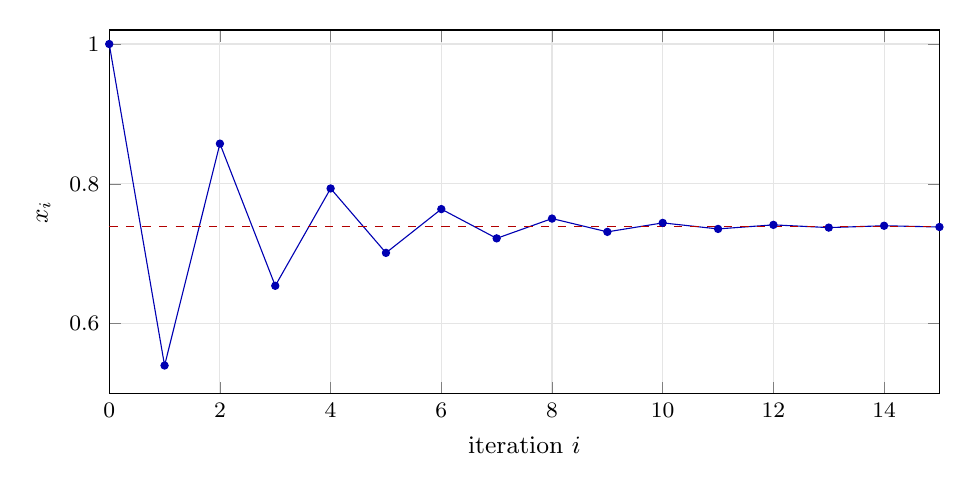
\begin{tikzpicture}
\begin{axis}[width=\linewidth, height=6.2cm, xmin=0, xmax=15, ymin=0.5, ymax=1.02, xlabel={iteration $i$}, ylabel={$x_i$}, grid=both, grid style={gray!20}]
\addplot[blue!70!black, mark=*, mark size=1.3pt] coordinates {(0.000000,1.000000) (1.000000,0.540302) (2.000000,0.857553) (3.000000,0.654290) (4.000000,0.793480) (5.000000,0.701369) (6.000000,0.763960) (7.000000,0.722102) (8.000000,0.750418) (9.000000,0.731404) (10.000000,0.744237) (11.000000,0.735605) (12.000000,0.741425) (13.000000,0.737507) (14.000000,0.740147) (15.000000,0.738369)};
\addplot[red!70!black, dashed] coordinates {(0,0.739085)(15,0.739085)};
\end{axis}
\end{tikzpicture}
\end{minipage}
\caption{Fixed-point iteration of $f(x)=\cos x$ from $x_0=1$ (original figure in the style of slide 24; values computed exactly). Left: cobweb diagram. Right: $x_i\to x^*\approx0.739085$.}
\label{fig:cobweb}
\end{figure}

\begin{intuition}
Fixed-point iteration is ``keep applying the rule until it stops changing anything''. Whether this works depends on the rule: with $f(x)=\cos x$ each step lands closer to $x^*$ (the cobweb spirals in), but for $f(x)=2x$ the iterates would run away from the fixed point $0$. The property that guarantees spiralling \emph{in} is that $f$ brings any two points closer together, which is exactly what the next section calls a contraction.
\end{intuition}
%=====================================================================
\section{Contractions \slides{25--28}}\label{sec:contr}
%=====================================================================
Convergence to a fixed point is possible thanks to the existence of \textbf{contraction mappings}.

\pdfnum{1}
\begin{definition}[Contraction]\label{def:contraction}
Let $(M,d)$ be a metric space. An operator $f:M\to M$ is a \emph{$k$-contraction} if there is $k\in[0,1)$ with
\[
d\big(f(x),f(y)\big)\le k\,d(x,y)\qquad\text{for all }x,y\in M .
\]
(On the slides: $\abs{f(x)-f(x')}\le k\abs{x-x'}$ for $k\in[0,1)$.)
\end{definition}

\pdfnum{2}
\begin{theorem}[Banach fixed-point theorem]\label{thm:banach}
A $k$-contraction on a non-empty \emph{complete} metric space has \emph{exactly one} fixed point $x^*$, and for any starting point $x_0$ the iteration $x_{i+1}=f(x_i)$ converges to it, with $d(x_i,x^*)\le k^i\,d(x_0,x^*)$.
\end{theorem}
\begin{proof}[Proof of uniqueness (this is the part on slide 25: ``a contraction mapping has at most one fixed point'')]
If $f(x)=x$ and $f(y)=y$ then $d(x,y)=d(f(x),f(y))\le k\,d(x,y)$, and since $k<1$ this forces $d(x,y)=0$, i.e.\ $x=y$.
\end{proof}
\emph{The existence of a fixed point, the convergence of the iteration and the rate $k^i$ are not proved on the slides; their proof is in Appendix~\ref{app:banach} (supplementary).}

\begin{intuition}
A contraction is a map that \emph{squeezes space}: any two points end up closer together after one application, by a factor of at least $k<1$. Two fixed points would stay at the same distance after applying $f$, which contradicts the squeezing, so there is at most one. Iterating $f$ keeps squeezing the whole space towards a single point, which is the fixed point; completeness just guarantees that this point exists inside the space instead of being a ``hole''. The rate $k^i$ is the geometric decay that all later bounds inherit.
\end{intuition}

\begin{figure}[htbp]
\centering
\begin{minipage}{0.52\linewidth}
\centering
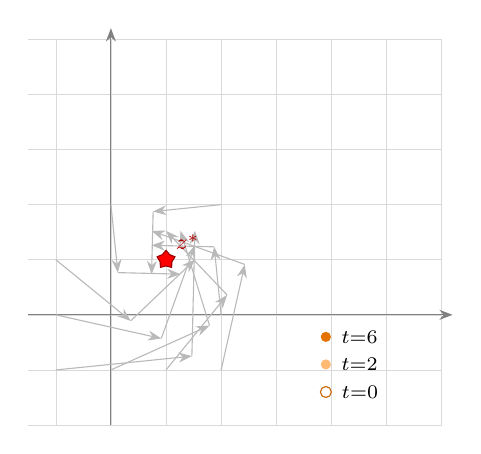
\begin{tikzpicture}[scale=0.7,
  c0/.style={circle, draw=orange!80!black, fill=white, inner sep=1.4pt},
  c2/.style={circle, fill=orange!55, inner sep=1.3pt},
  c6/.style={circle, fill=orange!90!black, inner sep=1.3pt}]
\draw[gray!30, very thin] (-1.5,-2) grid (6,5);
\draw[->, gray] (-1.5,0) -- (6.2,0); \draw[->, gray] (0,-2) -- (0,5.2);
\draw[->, gray!55] (-1.000,-1.000) -- (1.469,-0.749);
\draw[->, gray!55] (0.000,-1.000) -- (1.789,-0.194);
\draw[->, gray!55] (1.000,-1.000) -- (2.109,0.360);
\draw[->, gray!55] (2.000,-1.000) -- (2.429,0.914);
\draw[->, gray!55] (-1.000,0.000) -- (0.914,-0.429);
\draw[->, gray!55] (2.000,0.000) -- (1.874,1.234);
\draw[->, gray!55] (-1.000,1.000) -- (0.360,-0.109);
\draw[->, gray!55] (0.000,2.000) -- (0.126,0.766);
\draw[->, gray!55] (2.000,2.000) -- (0.766,1.874);
\draw[->, gray!55] (1.469,-0.749) -- (1.524,1.524);
\draw[->, gray!55] (1.789,-0.194) -- (1.262,1.524);
\draw[->, gray!55] (2.109,0.360) -- (1.000,1.524);
\draw[->, gray!55] (2.429,0.914) -- (0.738,1.524);
\draw[->, gray!55] (0.914,-0.429) -- (1.524,1.262);
\draw[->, gray!55] (1.874,1.234) -- (0.738,1.262);
\draw[->, gray!55] (0.360,-0.109) -- (1.524,1.000);
\draw[->, gray!55] (0.126,0.766) -- (1.262,0.738);
\draw[->, gray!55] (0.766,1.874) -- (0.738,0.738);
\node[star, star points=5, fill=red, draw=red!60!black, inner sep=1.6pt] at (1,1) {};
\node[red!70!black, font=\footnotesize, above right] at (1,1) {$z^*$};
\node[c0, label={[font=\scriptsize]right:$t{=}0$}] at (3.9,-1.4) {};
\node[c2, label={[font=\scriptsize]right:$t{=}2$}] at (3.9,-0.9) {};
\node[c6, label={[font=\scriptsize]right:$t{=}6$}] at (3.9,-0.4) {};
\end{tikzpicture}
\end{minipage}\hfill
\begin{minipage}{0.45\linewidth}
\centering
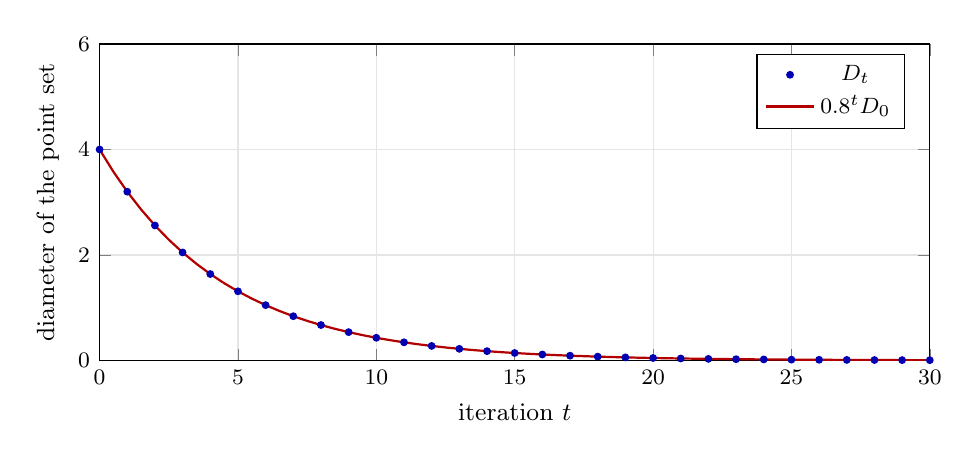
\begin{tikzpicture}
\begin{axis}[width=\linewidth, height=5.6cm, xmin=0, xmax=30, ymin=0, ymax=6, xlabel={iteration $t$}, ylabel={diameter of the point set}, grid=both, grid style={gray!20}, legend pos=north east]
\addplot[only marks, mark=*, mark size=1.2pt, blue!70!black] coordinates {(0.000000,4.000000) (1.000000,3.200000) (2.000000,2.560000) (3.000000,2.048000) (4.000000,1.638400) (5.000000,1.310720) (6.000000,1.048576) (7.000000,0.838861) (8.000000,0.671089) (9.000000,0.536871) (10.000000,0.429497) (11.000000,0.343597) (12.000000,0.274878) (13.000000,0.219902) (14.000000,0.175922) (15.000000,0.140737) (16.000000,0.112590) (17.000000,0.090072) (18.000000,0.072058) (19.000000,0.057646) (20.000000,0.046117) (21.000000,0.036893) (22.000000,0.029515) (23.000000,0.023612) (24.000000,0.018889) (25.000000,0.015112) (26.000000,0.012089) (27.000000,0.009671) (28.000000,0.007737) (29.000000,0.006190) (30.000000,0.004952)};
\addplot[red!70!black, thick, domain=0:30, samples=61] {4*0.8^x};
\legend{$D_t$, $0.8^t D_0$}
\end{axis}
\end{tikzpicture}
\end{minipage}
\caption{A contraction in $\R^2$ (original figure in the style of slide 26): $f(z)=0.8\,R_{30^\circ}z+c$ with unique fixed point $z^*$. Left: nine starting points and their images after $2$ and $6$ steps all collapse onto $z^*$. Right: the diameter of the point set decays exactly like $k^tD_0$ (here $f$ is a similarity, so the contraction inequality is tight).}
\label{fig:contraction}
\end{figure}

\begin{example}[{Why $\cos$ is a contraction on $[0,1]$}]\label{ex:cos}
\emph{(Added example connecting the cobweb of slide 24 to Banach's theorem; not on the slides.)} On $M=[0,1]$ (complete) $\cos$ maps into $[\cos1,1]\approx[0.540,1]\subset M$, and by the mean value theorem $\abs{\cos x-\cos y}=\abs{\sin\xi}\,\abs{x-y}\le\sin(1)\,\abs{x-y}$ with $\sin 1\approx0.841$. So $\cos$ is a $0.841$-contraction on $[0,1]$; Theorem~\ref{thm:banach} gives a unique fixed point ($x^*\approx0.739085$) and $\abs{x_i-x^*}\le0.841^i\abs{x_0-x^*}$. In \figref{fig:cobweb}, $x_0=1$ gives $\abs{x_5-x^*}\approx0.038$, comfortably below the bound $0.841^5\cdot0.261\approx0.110$.
\end{example}

\subsection{Contraction Operator \slides{27--28}}
In the simplest case the contraction can be an \emph{operator}, even as simple as a matrix $O$ acting on value vectors:
\[
\abs{OV-OV'}\le\gamma\abs{V-V'}
\]
(we can write $\gamma$ instead of $k$, since both lie in $[0,1)$). The slide's demo takes $O=\gamma I$, ``pure shrink'': every vector is scaled by $\gamma$, so the distance between $OV$ and $OV'$ is exactly $\gamma$ times the distance between $V$ and $V'$ (\figref{fig:operator}).

\begin{figure}[htbp]
\centering
\begin{minipage}{0.55\linewidth}
\centering
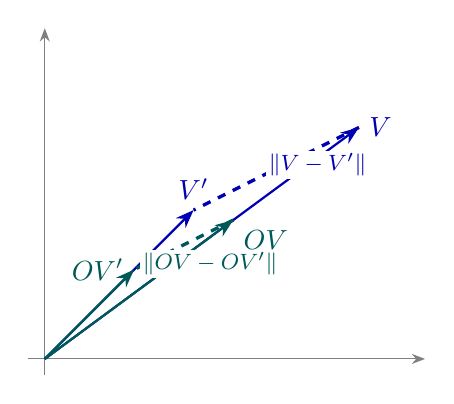
\begin{tikzpicture}[scale=1.05]
\draw[->, gray] (-0.2,0) -- (4.6,0); \draw[->, gray] (0,-0.2) -- (0,4.0);
\coordinate (V) at (3.8,2.8); \coordinate (W) at (1.8,1.8);
\coordinate (OV) at (2.28,1.68); \coordinate (OW) at (1.08,1.08);
\draw[->, thick, blue!70!black] (0,0) -- (V) node[right] {$V$};
\draw[->, thick, blue!70!black] (0,0) -- (W) node[above] {$V'$};
\draw[->, thick, teal!70!black] (0,0) -- (OV) node[below right] {$OV$};
\draw[->, thick, teal!70!black] (0,0) -- (OW) node[left] {$OV'$};
\draw[dashed, blue!70!black, very thick] (V) -- (W);
\draw[dashed, teal!70!black, very thick] (OV) -- (OW);
\node[blue!70!black, font=\footnotesize, fill=white, inner sep=1pt] at (3.3,2.35) {$\lVert V-V'\rVert$};
\node[teal!70!black, font=\footnotesize, fill=white, inner sep=1pt] at (2.0,1.15) {$\lVert OV-OV'\rVert$};
\end{tikzpicture}
\end{minipage}\hfill
\begin{minipage}{0.4\linewidth}
\centering
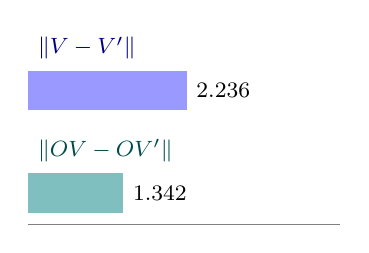
\begin{tikzpicture}[x=0.9cm]
  \fill[blue!40] (0,1.6) rectangle (2.236,2.1);
  \fill[teal!50] (0,0.3) rectangle (1.342,0.8);
  \node[anchor=west, font=\footnotesize] at (2.236,1.85) {2.236};
  \node[anchor=west, font=\footnotesize] at (1.342,0.55) {1.342};
  \node[anchor=south west, font=\footnotesize, blue!50!black] at (0,2.12) {$\lVert V-V'\rVert$};
  \node[anchor=south west, font=\footnotesize, teal!60!black] at (0,0.82) {$\lVert OV-OV'\rVert$};
  \draw[gray] (0,0.15) -- (4.4,0.15);
\end{tikzpicture}
\end{minipage}
\caption{Contraction operator $O=\gamma I$ with $\gamma=0.6$ (original figure in the style of slide 28; Euclidean norm). Applying $O$ shrinks the distance between any two value vectors from $2.236$ to $1.342=0.6\times2.236$.}
\label{fig:operator}
\end{figure}

\begin{intuition}
The point of this slide is the \emph{reading} of ``contraction'' for value functions: think of each value function as a point in $\R^{|\cS|}$ (one coordinate per state); an operator is a contraction when it makes two different value functions \emph{more similar}. The Bellman backups we are about to study are not as trivial as $\gamma I$, but they shrink distances in the same way, by at least a factor $\gamma$ in sup-norm.
\end{intuition}

%=====================================================================
\section{Iterative Policy Evaluation \slides{29--32}}\label{sec:itpe}
%=====================================================================
Instead of inverting a matrix, we exploit the fixed-point structure $V^\pi=r^\pi+\gamma P^\pi V^\pi$ and \emph{iterate} it. We assume rewards are in $[0,1]$.

\begin{algorithm}[Iterative policy evaluation]\label{alg:pe}
\emph{Input:} an MDP $(\cS,\cA,p,r,\gamma)$ and a policy $\pi$.\par
\begin{enumerate}[label=\arabic*.,leftmargin=*]
  \item Initialise $V_0\in[0,1/(1-\gamma)]^{|\cS|}$ (typically $V_0=0$).
  \item Until convergence: $V_{i+1}=r^\pi+\gamma P^\pi V_i$ \quad (matrix form: all states are updated at once).
\end{enumerate}
In operator notation, $V_{i+1}=\Bpi V_i$: this is the \emph{Bellman expectation backup}.
\end{algorithm}
(In the companion note: ``repeat $V_{i+1}=\Bpi V_i$ until $\norm{V_{i+1}-V_i}$ is small.'')

\textbf{Why initialise in $[0,1/(1-\gamma)]$?} Under the assumption $r(s,a)\in[0,1]$, the maximum possible value is $1+\gamma+\gamma^2+\dots=1/(1-\gamma)$ (Fact~\ref{fact:range}). There is no reason to initialise higher than that, since no true value lives there.

\pdfnum{3}
\begin{definition}[Bellman operators]\label{def:bellman}
For a policy $\pi$, a value function $V$ and a state-action function $Q$:
\begin{align*}
(\Bpi V)(s)&=r(s,\pi(s))+\gamma\,\E_{s'\sim p(\cdot\mid s,\pi(s))}\big[V(s')\big] &&\text{(expectation backup, slide 32)},\\
(\Bell V)(s)&=\max_a\Big[r(s,a)+\gamma\,\E_{s'\sim p(\cdot\mid s,a)}\big[V(s')\big]\Big] &&\text{(optimality backup, slide 44)},\\
(\Bell Q)(s,a)&=r(s,a)+\gamma\,\E_{s'\sim p(\cdot\mid s,a)}\Big[\max_{a'}Q(s',a')\Big] &&\text{(on $Q$, slide 48)}.
\end{align*}
$\Bpi$ is \emph{affine} ($\Bpi V=r^\pi+\gamma P^\pi V$); $\Bell$ is \emph{not} linear, because of the maximum. (Part of the literature writes $T$ for $\Bell$.)
\end{definition}

\begin{intuition}
A ``backup'' is one round of ``look one step ahead and update''. The expectation backup $\Bpi$ asks: \emph{if I act according to $\pi$ for one step and then trust my current guess $V$, what is the value of each state?} The optimality backup $\Bell$ asks the same but lets me \emph{pick the best action} in the first step. Facts~\ref{fact:bexp} and \ref{fact:bopt} say precisely that $V^\pi$ and $V^*$ are the states of the world these backups leave untouched.
\end{intuition}

\begin{example}[Iterative evaluation on the two-state MDP]\label{ex:pe}
For $\pi=(a,a)$ in Example~\ref{ex:toy} and $V_0=0$ (so $\norm{V_0-V^\pi}=8.594$):
\begin{center}
\begin{tabular}{@{}rcccc@{}}
\toprule
$i$ & $V_i(s_1)$ & $V_i(s_2)$ & $\norm{V_i-V^\pi}$ & $\gamma^i\norm{V_0-V^\pi}$\\
\midrule
0 & 0.000 & 0.000 & 8.594 & 8.594 \\
1 & 0.000 & 1.000 & 7.594 & 7.734 \\
2 & 0.450 & 1.810 & 6.784 & 6.961 \\
3 & 1.017 & 2.507 & 6.087 & 6.265 \\
4 & 1.586 & 3.122 & 5.472 & 5.638 \\
5 & 2.118 & 3.671 & 4.922 & 5.075 \\
6 & 2.605 & 4.165 & 4.429 & 4.567 \\
7 & 3.046 & 4.608 & 3.986 & 4.110 \\
8 & 3.444 & 5.006 & 3.587 & 3.699 \\
9 & 3.803 & 5.365 & 3.229 & 3.329 \\
10 & 4.126 & 5.688 & 2.906 & 2.996 \\
11 & 4.416 & 5.979 & 2.615 & 2.697 \\
12 & 4.678 & 6.240 & 2.354 & 2.427 \\
13 & 4.913 & 6.476 & 2.118 & 2.184 \\
14 & 5.125 & 6.687 & 1.906 & 1.966 \\
15 & 5.315 & 6.878 & 1.716 & 1.769 \\
\bottomrule
\end{tabular}
\end{center}
The first sweep gives $V_1=r^\pi=(0,1)$; each later sweep propagates reward information one step further. The true error always stays below the geometric bound (last column), as proved next.
\end{example}

%=====================================================================
\section{Iterative Policy Evaluation Theorem \slides{33--37}}\label{sec:thm4}
%=====================================================================
The slides' claim is that, for any two value functions $U$ and $V$ and for all $s\in\cS$,
\[
\abs{(\Bpi U)(s)-(\Bpi V)(s)}\le\gamma\norm{U-V},\qquad\norm{V}=\max_s\abs{V(s)}
\]
(``the largest difference between state values'', worst case scenario to infinity). The companion note packages this together with the analogous claim for $\Bell$ (proved later, slides 44--47):

\pdfnum{4}
\begin{theorem}[Both operators are $\gamma$-contractions in the sup-norm]\label{thm:contraction}
For all value functions $U,V$:
\[
\text{(i)}\ \ \norm{\Bpi U-\Bpi V}\le\gamma\norm{U-V},\qquad
\text{(ii)}\ \ \norm{\Bell U-\Bell V}\le\gamma\norm{U-V}.
\]
The same holds for $\Bell$ acting on state-action functions $Q$.
\end{theorem}
\begin{proof}[Proof of (i), as on slides 33--37]
For $\Bpi$ the rewards cancel. For every state $s$,
\begin{align*}
\abs{(\Bpi U)(s)-(\Bpi V)(s)}
&=\gamma\,\Big|\E_{s'}\big[U(s')-V(s')\big]\Big|\\
&\le\gamma\,\E_{s'}\abs{U(s')-V(s')} &&\text{(Jensen: $\abs{\cdot}$ is convex)}\\
&\le\gamma\,\norm{U-V} &&\text{(an average is at most the maximum).}
\end{align*}
The inequality holds for every $s$, so also for the state where the left-hand side is largest; taking the maximum over $s$ gives (i). The proof of (ii) is in Section~\ref{sec:optcontr}.
\end{proof}

\begin{intuition}
Two things happen in the proof. First, both backups use the \emph{same} rewards, so these cancel: the only thing that differs is the next-state values, scaled by $\gamma$. Second, the next-state values are \emph{averaged} by probabilities that sum to one, and an average of numbers each at most $\norm{U-V}$ in size cannot exceed $\norm{U-V}$. So no state can end up further apart than $\gamma$ times the worst gap before. As the slide remarks, we are not secretly using the sup-norm on the left-hand side: the bound holds \emph{for each state}, including the one with the largest difference.
\end{intuition}

Slide 34 draws the conclusion: \emph{hence the Bellman expectation backup is a contraction mapping and $V^\pi$ is its fixed point}. This follows from Theorem~\ref{thm:banach} applied to $\Bpi$ on $(\R^{|\cS|},\norm{\cdot})$, which is complete (a finite-dimensional normed space): by Fact~\ref{fact:bexp}, $\Bpi V^\pi=V^\pi$, so $V^\pi$ is a fixed point, and by Banach's uniqueness it is the only one. (This is part (a) of Corollary~\ref{cor:fixed}, stated in full in the Value Iteration section.)

%=====================================================================
\section{Iterative Policy Evaluation: Iterations \slide{38}}\label{sec:peiters}
%=====================================================================
\pdfnum{6}
\begin{corollary}[Convergence and cost of iterative policy evaluation]\label{cor:pe}
$\norm{V_i-V^\pi}\le\gamma^i\norm{V_0-V^\pi}$, so $\norm{V_i-V^\pi}\le\epsilon$ after
\[
i\;\ge\;\frac{\ln\!\big(\norm{V_0-V^\pi}/\epsilon\big)}{\ln(1/\gamma)}
\]
iterations, each costing $O(|\cS|^2)$ arithmetic operations. Hence an $\epsilon$-accurate value function costs $O\big(|\cS|^2\ln(1/\epsilon)\big)$ (treating $\gamma$ and $\norm{V_0-V^\pi}$ as constants).
\end{corollary}
\begin{proof}
The rate is Theorem~\ref{thm:banach} with $k=\gamma$, applied to $\Bpi$ whose unique fixed point is $V^\pi$. Solving $\gamma^i\norm{V_0-V^\pi}\le\epsilon$ for $i$ (take logarithms; $\ln\gamma=-\ln(1/\gamma)<0$ flips the inequality) gives the count. Each sweep updates $|\cS|$ states and each update averages over $|\cS|$ successors, i.e.\ one matrix--vector product $P^\pi V_i$.
\end{proof}

\begin{figure}[htbp]
\centering
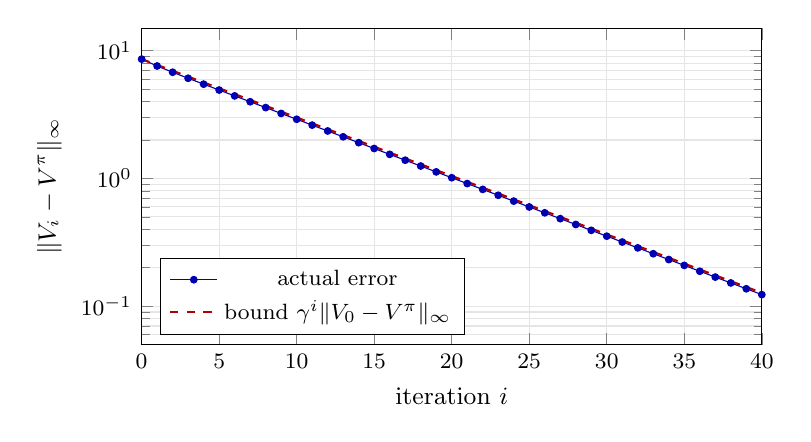
\begin{tikzpicture}
\begin{axis}[width=0.78\linewidth, height=5.6cm, xmin=0, xmax=40, ymode=log, ymin=0.05, ymax=15, xlabel={iteration $i$}, ylabel={$\norm{V_i-V^\pi}$}, grid=both, grid style={gray!20}, legend pos=south west]
\addplot[blue!70!black, mark=*, mark size=1.2pt] coordinates {(0.000000,8.593750) (1.000000,7.593750) (2.000000,6.783750) (3.000000,6.087150) (4.000000,5.471874) (5.000000,4.922325) (6.000000,4.429242) (7.000000,3.986012) (8.000000,3.587300) (9.000000,3.228531) (10.000000,2.905663) (11.000000,2.615092) (12.000000,2.353581) (13.000000,2.118222) (14.000000,1.906400) (15.000000,1.715759) (16.000000,1.544184) (17.000000,1.389765) (18.000000,1.250789) (19.000000,1.125710) (20.000000,1.013139) (21.000000,0.911825) (22.000000,0.820642) (23.000000,0.738578) (24.000000,0.664720) (25.000000,0.598248) (26.000000,0.538423) (27.000000,0.484581) (28.000000,0.436123) (29.000000,0.392511) (30.000000,0.353260) (31.000000,0.317934) (32.000000,0.286140) (33.000000,0.257526) (34.000000,0.231774) (35.000000,0.208596) (36.000000,0.187737) (37.000000,0.168963) (38.000000,0.152067) (39.000000,0.136860) (40.000000,0.123174)};
\addplot[red!70!black, dashed, thick, domain=0:40, samples=41] {8.59375*0.9^x};
\legend{actual error, bound $\gamma^i\norm{V_0-V^\pi}$}
\end{axis}
\end{tikzpicture}
\caption{Iterative policy evaluation on Example~\ref{ex:toy} with $\pi=(a,a)$, $\gamma=0.9$, $V_0=0$. On a log scale the error is a straight line: geometric convergence. The error decays geometrically and remains below the contraction bound.}
\label{fig:pe_err}
\end{figure}

\begin{intuition}
\emph{Worked numbers.} With $\gamma=0.9$, $\epsilon=0.01$ and $\norm{V_0-V^\pi}=8.594$: $i\ge\ln(859.4)/\ln(1/0.9)=6.756/0.1054=64.1$, so $65$ sweeps (indeed $0.9^{65}\cdot8.594\approx0.009$). Each sweep is only $|\cS|^2=4$ multiplications here. The \emph{accuracy} costs only a logarithm ($10\times$ smaller $\epsilon$ adds $\ln 10/\ln(1/\gamma)\approx22$ sweeps), while the \emph{horizon} $\ln(1/\gamma)\approx1-\gamma$ drives the cost. Compared with $O(|\cS|^3)$ for exact evaluation, iteration wins when $|\cS|$ is large and $\epsilon$ is moderate.
\end{intuition}
%=====================================================================
\section{How to Find the Optimal Policy? \slides{39--43}}
%=====================================================================
Now what we are really interested in is finding the optimal policy $\pi^*$.

\textbf{Naive approach} (slides 40--42): we know how to do policy evaluation, so
\begin{itemize}
  \item for each possible policy, for all states,
  \item do policy evaluation and compute $V^\pi(s)$,
  \item choose $\pi'$ such that $V^{\pi'}(s)\ge V^\pi(s)$ (keep the best).
\end{itemize}
If we use exact policy evaluation the cost is $O\big(|\cA|^{|\cS|}\,|\cS|^3\big)$: $|\cA|^{|\cS|}$ policies, each needing a cubic solve.

\begin{intuition}
The slide's horrified emoji is justified. The number of deterministic policies grows \emph{exponentially} in the number of states: for $|\cA|=2$, $|\cS|=10$ there are $1024$ policies (about $10^6$ operations in total), but for $|\cS|=30$ there are $2^{30}\approx10^9$ policies and about $2.9\times10^{13}$ operations. Enumeration treats the policies as unrelated black boxes. The better idea (slide 43): \textbf{let's use the Bellman optimality equation!} Rather than searching over policies, search for the one function $V^*$ (or $Q^*$) that satisfies it, and read the policy off with an $\argmax$ (Fact~\ref{fact:bopt}).
\end{intuition}

%=====================================================================
\section{The Bellman Optimality Backup is a Contraction \slides{44--47}}\label{sec:optcontr}
%=====================================================================
Set $\gamma<1$ and use the sup-norm $\norm{V}=\max_s\abs{V(s)}$. Define the (non-linear) operator $\Bell V$ as the Bellman optimality equation applied to $V$ (Definition~\ref{def:bellman}):
\[
(\Bell V)(s)=\max_a\Big[r(s,a)+\gamma\sum_{s'\in\cS}p(s'\mid s,a)\,V(s')\Big].
\]
We need one elementary fact about maxima, used implicitly on the slides:

\begin{lemma}[The maximum is 1-Lipschitz]\label{lem:max}
For any two functions $f,g$ on a finite set of actions, $\big|\max_af(a)-\max_ag(a)\big|\le\max_a\abs{f(a)-g(a)}$.
\end{lemma}
\begin{proof}
Let $a_f$ attain $\max_af$. Then $\max_af-\max_ag\le f(a_f)-g(a_f)\le\max_a\abs{f(a)-g(a)}$. Exchanging the roles of $f$ and $g$ gives the other sign.
\end{proof}

\begin{proof}[Proof of Theorem~\ref{thm:contraction}\,(ii), following slides 45--47]
Fix two value functions $V_k,V_j$ and a state $s$. Using Lemma~\ref{lem:max} with $f(a)=r(s,a)+\gamma\sum_{s'}p(s'\mid s,a)V_k(s')$ and $g$ the same with $V_j$, the reward terms cancel:
\begin{align*}
\big|(\Bell V_k)(s)-(\Bell V_j)(s)\big|
&\le\max_a\Big|\gamma\sum_{s'}p(s'\mid s,a)\big(V_k(s')-V_j(s')\big)\Big|\\
&\le\max_a\gamma\sum_{s'}p(s'\mid s,a)\,\norm{V_k-V_j}\\
&=\gamma\norm{V_k-V_j},
\end{align*}
where the second step bounds each $\abs{V_k(s')-V_j(s')}$ by the sup-norm, and the last equality uses $\sum_{s'}p(s'\mid s,a)=1$. Taking the maximum over $s$ gives $\norm{\Bell V_k-\Bell V_j}\le\gamma\norm{V_k-V_j}$.
\end{proof}

\begin{intuition}
If you apply $\Bell$ to two different value functions, \emph{the distance between them shrinks} (slide 46): $\Bell$ makes value functions closer by at least a factor $\gamma$ (slide 47). The new ingredient compared with the expectation backup is the $\max$, and Lemma~\ref{lem:max} says it cannot amplify differences: changing a few action values by at most $\delta$ changes the best of them by at most $\delta$. So even though $\Bell$ is non-linear, it inherits the same squeezing property as $\Bpi$.
\end{intuition}

%=====================================================================
\section{Bellman Operator for $Q$ \slide{48}}
%=====================================================================
Since $Q:\cS\times\cA\to\R$, also $\Bell Q:\cS\times\cA\to\R$:
\[
(\Bell Q)(s,a)=r(s,a)+\gamma\,\E_{s'\sim p(\cdot\mid s,a)}\Big[\max_{a'}Q(s',a')\Big],
\]
and the norm is now $\norm{Q}=\max_{s,a}\abs{Q(s,a)}$.

\begin{proof}[Proof of the last claim of Theorem~\ref{thm:contraction} (the $Q$-version)]
Rewards cancel, and the maximum now sits \emph{inside} the expectation. For every $(s,a)$,
\[
\abs{(\Bell Q)(s,a)-(\Bell Q')(s,a)}
=\gamma\Big|\E_{s'}\big[\max_{a'}Q(s',a')-\max_{a'}Q'(s',a')\big]\Big|
\le\gamma\,\E_{s'}\max_{a'}\abs{Q(s',a')-Q'(s',a')}
\le\gamma\norm{Q-Q'},
\]
using $\abs{\E X}\le\E\abs{X}$, Lemma~\ref{lem:max}, and that an average is at most the maximum. Taking the maximum over $(s,a)$ finishes the proof.
\end{proof}

\begin{intuition}
Nothing new happens: the $Q$-table has $|\cS||\cA|$ entries instead of $|\cS|$, and the same ``rewards cancel, averages cannot exceed the worst case'' argument applies. Working with $Q$ is convenient because a policy can be read off from $Q$ without a model: $\argmax_aQ(s,a)$.
\end{intuition}

%=====================================================================
\section{Value Iteration \slides{49--53}}\label{sec:vi}
%=====================================================================
We can obtain $Q^*=\Bell Q^*$, since $Q^*$ is a fixed point of $Q=\Bell Q$ (and all of this also holds for $V^*$).

\pdfnum{5}
\begin{corollary}[What the fixed points are]\label{cor:fixed}
\emph{(a)} $V^\pi$ is the unique fixed point of $\Bpi$; \emph{(b)} $V^*$ is the unique fixed point of $\Bell$ on value functions; \emph{(c)} $Q^*$ is the unique fixed point of $\Bell$ on state-action functions.
\end{corollary}
\begin{proof}
Fact~\ref{fact:bexp} says $\Bpi V^\pi=V^\pi$ and Fact~\ref{fact:bopt} says $\Bell V^*=V^*$ and $\Bell Q^*=Q^*$, so each is a fixed point. The spaces $(\R^{|\cS|},\norm{\cdot})$ and $(\R^{|\cS||\cA|},\norm{\cdot})$ are complete, and Theorem~\ref{thm:contraction} says the operators are $\gamma$-contractions, so Theorem~\ref{thm:banach} says each has only one fixed point.
\end{proof}
\emph{(This also re-proves Fact~\ref{fact:uniq}, slide 11, in one line: any $V$ with $\Bell V=V$ is the fixed point of $\Bell$, hence equals $V^*$; this is what the long unrolling argument in L03 did by hand.)}

\begin{algorithm}[Value iteration]\label{alg:vi}
\emph{Input:} an MDP $(\cS,\cA,p,r,\gamma)$.\par
\begin{enumerate}[label=\arabic*.,leftmargin=*]
  \item Initialise $Q_0$ with entries in $[0,1/(1-\gamma)]$ (typically $Q_0=0$).
  \item Until convergence, for all states and actions:
  \[
  Q_{i+1}(s,a)=(\Bell Q_i)(s,a)=r(s,a)+\gamma\sum_{s'}p(s'\mid s,a)\max_{a'}Q_i(s',a').
  \]
  \item Return the greedy policy $\pi_i(s)\in\argmax_aQ_i(s,a)$ (slide 54).
\end{enumerate}
\end{algorithm}

\pdfnum{7}
\begin{theorem}[Value iteration converges geometrically]\label{thm:vi}
$\norm{Q_i-Q^*}\le\gamma^i\norm{Q_0-Q^*}$, and each iteration costs $O(|\cS|^2|\cA|)$.
\end{theorem}
\begin{proof}
By Theorem~\ref{thm:contraction} and Corollary~\ref{cor:fixed}(c), $\norm{Q_{i+1}-Q^*}=\norm{\Bell Q_i-\Bell Q^*}\le\gamma\norm{Q_i-Q^*}$, and induction gives $\norm{Q_i-Q^*}\le\gamma^i\norm{Q_0-Q^*}$ (slide 51). For the cost (slide 53): compute $m_i(s')=\max_{a'}Q_i(s',a')$ once per state ($|\cS||\cA|$ operations); then each of the $|\cS||\cA|$ entries needs a sum over $|\cS|$ successors, using the shared $m_i$. Total $O(|\cS|^2|\cA|)$.
\end{proof}

\begin{intuition}
Value iteration is the same fixed-point iteration as in the cobweb picture, run on the \emph{vector} $Q$ with the operator $\Bell$: start from any guess, repeatedly ``look one step ahead and take the best action'', and the guess is pulled towards $Q^*$ at geometric speed. No search over policies is needed: compare $O(|\cS|^2|\cA|)$ per iteration, for about $\ln(1/\epsilon)/(1-\gamma)$ iterations, with the $|\cA|^{|\cS|}$ of the naive approach. A useful way to see how it works: after $i$ iterations, $Q_i(s,a)$ is the best total discounted reward you can collect in the first $i$ steps (from a terminal value of $Q_0$), so reward information spreads one step per iteration.
\end{intuition}

\begin{figure}[htbp]
\centering
\begin{minipage}{0.49\linewidth}
\centering
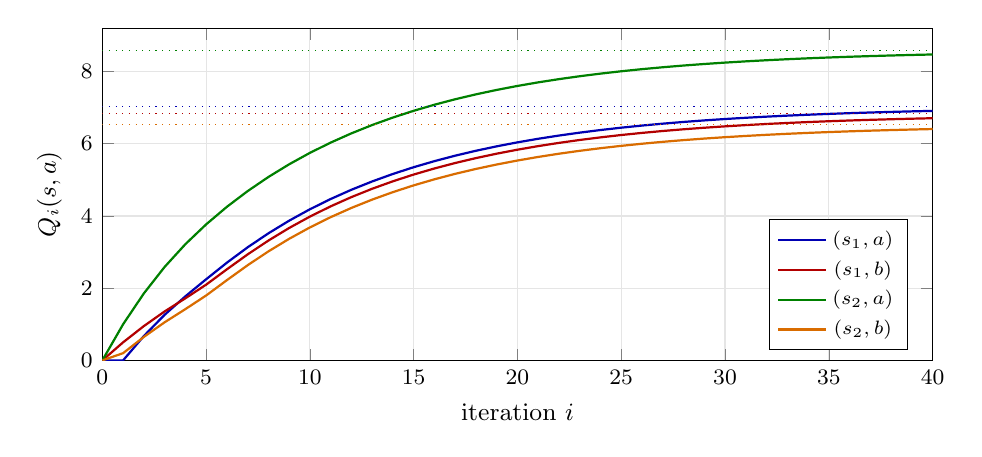
\begin{tikzpicture}
\begin{axis}[width=\linewidth, height=5.8cm, xmin=0, xmax=40, ymin=0, ymax=9.2, xlabel={iteration $i$}, ylabel={$Q_i(s,a)$}, grid=both, grid style={gray!20}, legend style={at={(0.97,0.03)}, anchor=south east, font=\scriptsize}]
\addplot[blue!70!black, thick] coordinates {(0.000000,0.000000) (1.000000,0.000000) (2.000000,0.675000) (3.000000,1.262250) (4.000000,1.774372) (5.000000,2.246689) (6.000000,2.705932) (7.000000,3.131547) (8.000000,3.519027) (9.000000,3.869353) (10.000000,4.185220) (11.000000,4.469707) (12.000000,4.725819) (13.000000,4.956347) (14.000000,5.163832) (15.000000,5.350572) (16.000000,5.518639) (17.000000,5.669900) (18.000000,5.806035) (19.000000,5.928556) (20.000000,6.038826) (21.000000,6.138068) (22.000000,6.227386) (23.000000,6.307773) (24.000000,6.380120) (25.000000,6.445233) (26.000000,6.503835) (27.000000,6.556577) (28.000000,6.604044) (29.000000,6.646764) (30.000000,6.685213) (31.000000,6.719817) (32.000000,6.750960) (33.000000,6.778989) (34.000000,6.804215) (35.000000,6.826919) (36.000000,6.847352) (37.000000,6.865742) (38.000000,6.882292) (39.000000,6.897188) (40.000000,6.910594)};
\addplot[red!70!black, thick] coordinates {(0.000000,0.000000) (1.000000,0.500000) (2.000000,0.950000) (3.000000,1.355000) (4.000000,1.719500) (5.000000,2.096935) (6.000000,2.522020) (7.000000,2.935339) (8.000000,3.318392) (9.000000,3.667124) (10.000000,3.982418) (11.000000,4.266698) (12.000000,4.522736) (13.000000,4.753237) (14.000000,4.960713) (15.000000,5.147449) (16.000000,5.315515) (17.000000,5.466775) (18.000000,5.602910) (19.000000,5.725431) (20.000000,5.835701) (21.000000,5.934943) (22.000000,6.024261) (23.000000,6.104648) (24.000000,6.176995) (25.000000,6.242108) (26.000000,6.300710) (27.000000,6.353452) (28.000000,6.400919) (29.000000,6.443639) (30.000000,6.482088) (31.000000,6.516692) (32.000000,6.547835) (33.000000,6.575864) (34.000000,6.601090) (35.000000,6.623794) (36.000000,6.644227) (37.000000,6.662617) (38.000000,6.679167) (39.000000,6.694063) (40.000000,6.707469)};
\addplot[green!50!black, thick] coordinates {(0.000000,0.000000) (1.000000,1.000000) (2.000000,1.855000) (3.000000,2.588050) (4.000000,3.218271) (5.000000,3.766493) (6.000000,4.253061) (7.000000,4.688513) (8.000000,5.079535) (9.000000,5.431136) (10.000000,5.747462) (11.000000,6.032114) (12.000000,6.288286) (13.000000,6.518835) (14.000000,6.726328) (15.000000,6.913070) (16.000000,7.081139) (17.000000,7.232400) (18.000000,7.368535) (19.000000,7.491056) (20.000000,7.601326) (21.000000,7.700568) (22.000000,7.789886) (23.000000,7.870273) (24.000000,7.942620) (25.000000,8.007733) (26.000000,8.066335) (27.000000,8.119077) (28.000000,8.166544) (29.000000,8.209264) (30.000000,8.247713) (31.000000,8.282317) (32.000000,8.313460) (33.000000,8.341489) (34.000000,8.366715) (35.000000,8.389419) (36.000000,8.409852) (37.000000,8.428242) (38.000000,8.444792) (39.000000,8.459688) (40.000000,8.473094)};
\addplot[orange!85!black, thick] coordinates {(0.000000,0.000000) (1.000000,0.200000) (2.000000,0.650000) (3.000000,1.055000) (4.000000,1.419500) (5.000000,1.796935) (6.000000,2.222020) (7.000000,2.635339) (8.000000,3.018392) (9.000000,3.367124) (10.000000,3.682418) (11.000000,3.966698) (12.000000,4.222736) (13.000000,4.453237) (14.000000,4.660713) (15.000000,4.847449) (16.000000,5.015515) (17.000000,5.166775) (18.000000,5.302910) (19.000000,5.425431) (20.000000,5.535701) (21.000000,5.634943) (22.000000,5.724261) (23.000000,5.804648) (24.000000,5.876995) (25.000000,5.942108) (26.000000,6.000710) (27.000000,6.053452) (28.000000,6.100919) (29.000000,6.143639) (30.000000,6.182088) (31.000000,6.216692) (32.000000,6.247835) (33.000000,6.275864) (34.000000,6.301090) (35.000000,6.323794) (36.000000,6.344227) (37.000000,6.362617) (38.000000,6.379167) (39.000000,6.394063) (40.000000,6.407469)};
\addplot[blue!70!black, dotted] coordinates {(0,7.03125)(40,7.03125)};
\addplot[red!70!black, dotted] coordinates {(0,6.828125)(40,6.828125)};
\addplot[green!50!black, dotted] coordinates {(0,8.59375)(40,8.59375)};
\addplot[orange!85!black, dotted] coordinates {(0,6.528125)(40,6.528125)};
\legend{{$(s_1,a)$},{$(s_1,b)$},{$(s_2,a)$},{$(s_2,b)$}}
\end{axis}
\end{tikzpicture}
\end{minipage}\hfill
\begin{minipage}{0.49\linewidth}
\centering
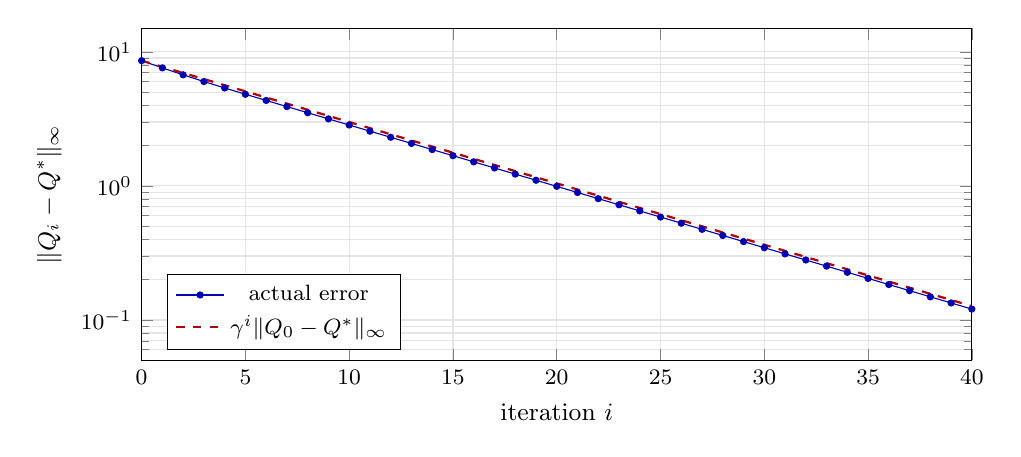
\begin{tikzpicture}
\begin{axis}[width=\linewidth, height=5.8cm, xmin=0, xmax=40, ymode=log, ymin=0.05, ymax=15, xlabel={iteration $i$}, ylabel={$\norm{Q_i-Q^*}$}, grid=both, grid style={gray!20}, legend pos=south west]
\addplot[blue!70!black, mark=*, mark size=1.1pt] coordinates {(0.000000,8.593750) (1.000000,7.593750) (2.000000,6.738750) (3.000000,6.005700) (4.000000,5.375479) (5.000000,4.827257) (6.000000,4.340689) (7.000000,3.905237) (8.000000,3.514215) (9.000000,3.162614) (10.000000,2.846288) (11.000000,2.561636) (12.000000,2.305464) (13.000000,2.074915) (14.000000,1.867422) (15.000000,1.680680) (16.000000,1.512611) (17.000000,1.361350) (18.000000,1.225215) (19.000000,1.102694) (20.000000,0.992424) (21.000000,0.893182) (22.000000,0.803864) (23.000000,0.723477) (24.000000,0.651130) (25.000000,0.586017) (26.000000,0.527415) (27.000000,0.474673) (28.000000,0.427206) (29.000000,0.384486) (30.000000,0.346037) (31.000000,0.311433) (32.000000,0.280290) (33.000000,0.252261) (34.000000,0.227035) (35.000000,0.204331) (36.000000,0.183898) (37.000000,0.165508) (38.000000,0.148958) (39.000000,0.134062) (40.000000,0.120656)};
\addplot[red!70!black, dashed, thick, domain=0:40, samples=41] {8.59375*0.9^x};
\legend{actual error, $\gamma^i\norm{Q_0-Q^*}$}
\end{axis}
\end{tikzpicture}
\end{minipage}
\caption{Value iteration on Example~\ref{ex:toy} ($\gamma=0.9$, $Q_0=0$), in the spirit of the demo on slide 52. Left: the four Q-values converge to $Q^*$ (dotted lines). Right: the error stays below the geometric bound of Theorem~\ref{thm:vi}.}
\label{fig:vi}
\end{figure}

\begin{example}[First iterations of value iteration]\label{ex:vi}
$Q_1=r$ (from $Q_0=0$). Then, e.g., $Q_2(s_1,a)=0+0.9\,(0.5\cdot\max Q_1(s_1,\cdot)+0.5\cdot\max Q_1(s_2,\cdot))=0.9(0.5\cdot0.5+0.5\cdot1)=0.675$, matching the table in Example~\ref{ex:greedy}. The fixed point is $Q^*=\begin{pmatrix}7.03125&6.828125\\8.59375&6.528125\end{pmatrix}$ (rows $s_1,s_2$; columns $a,b$), so $V^*=(7.03125,\,8.59375)$ and $\pi^*=(a,a)$.
\end{example}

%=====================================================================
\section{Policy from Value Iteration \slides{54--65}}\label{sec:greedy}
%=====================================================================
We know that $\pi^*(s)=\argmax_aQ^*(s,a)$, and since $Q_i(s,a)\approx Q^*(s,a)$ we can choose
\[
\pi_i(s)=\argmax_aQ_i(s,a).
\]
\textbf{What is the quality of such a policy?} For all states,

\pdfnum{8}
\begin{theorem}[Quality of the greedy policy]\label{thm:greedy}
Let $\pi_i(s)\in\argmax_aQ_i(s,a)$. Then for every state $s$,
\[
V^{\pi_i}(s)\;\ge\;V^*(s)-\frac{2\norm{Q_i-Q^*}}{1-\gamma}\;\ge\;V^*(s)-\frac{2\gamma^i\norm{Q_0-Q^*}}{1-\gamma}.
\]
\end{theorem}
\begin{proof}
Write $\varepsilon=\norm{Q_i-Q^*}$ and fix $s$. Using $V^{\pi_i}(s)=Q^{\pi_i}(s,\pi_i(s))$ and $V^*(s)=Q^*(s,\pi^*(s))$ (slide 56), add and subtract $Q^*(s,\pi_i(s))$ (slide 57):
\[
V^{\pi_i}(s)-V^*(s)=\underbrace{\big[Q^{\pi_i}(s,\pi_i(s))-Q^*(s,\pi_i(s))\big]}_{\text{(I)}}+\underbrace{\big[Q^*(s,\pi_i(s))-Q^*(s,\pi^*(s))\big]}_{\text{(II)}}.
\]
\emph{Term (I).} The two $Q$'s share the same reward term, which cancels (slide 58), so
\[
\text{(I)}=\gamma\,\E_{s'\sim p(\cdot\mid s,\pi_i(s))}\big[V^{\pi_i}(s')-V^*(s')\big].
\]
\emph{Term (II).} Insert $Q_i$ twice (slides 59--62):
\[
\text{(II)}=\underbrace{\big[Q^*(s,\pi_i(s))-Q_i(s,\pi_i(s))\big]}_{\ge-\varepsilon}+\underbrace{\big[Q_i(s,\pi_i(s))-Q_i(s,\pi^*(s))\big]}_{\ge0}+\underbrace{\big[Q_i(s,\pi^*(s))-Q^*(s,\pi^*(s))\big]}_{\ge-\varepsilon}\ \ge\ -2\varepsilon.
\]
The middle bracket is non-negative because $\pi_i$ maximises $Q_i$; the outer two are each at least $-\varepsilon$ by definition of $\varepsilon$.

\emph{Putting it together.} Let $\delta=\min_s\big[V^{\pi_i}(s)-V^*(s)\big]\le0$ (no policy beats $V^*$). Taking the state attaining the minimum, and bounding the expectation in (I) below by $\delta$,
\[
\delta\ge\gamma\delta-2\varepsilon\ \Longrightarrow\ \delta(1-\gamma)\ge-2\varepsilon\ \Longrightarrow\ \delta\ge-\frac{2\varepsilon}{1-\gamma}.
\]
This is the first inequality (it holds for every $s$ since $\delta$ is the minimum over $s$). The second inequality is Theorem~\ref{thm:vi}.
\end{proof}

\begin{remark}[The slides' ``repeat'' version, slides 63--65]
The slides stop at $V^{\pi_i}(s)-V^*(s)\ge\gamma\,\E_{s'}[V^{\pi_i}(s')-V^*(s')]-2\gamma^i\norm{Q_0-Q^*}$, using $\norm{Q_i-Q^*}\le\gamma^i\norm{Q_0-Q^*}$ twice, and then say ``repeat and get $1/(1-\gamma)$'': plugging the same bound into the expectation on the right again and again produces the geometric series $2\gamma^i\norm{Q_0-Q^*}\,(1+\gamma+\gamma^2+\cdots)=2\gamma^i\norm{Q_0-Q^*}/(1-\gamma)$. The $\delta$-trick above is the same argument written in one line.
\end{remark}

\begin{intuition}
\emph{Why a factor 2?} The greedy choice compares actions using $Q_i$ instead of $Q^*$; each of the two actions being compared (the one we pick and the true best) can be mis-valued by up to $\varepsilon$, in opposite directions, so the \emph{one-step} regret is up to $2\varepsilon$. \emph{Why $1/(1-\gamma)$?} A one-step mistake is not a one-time cost: the policy keeps following the same imperfect scores in all later states, so mistakes accumulate over the whole effective horizon. Note the guarantee is about the \emph{policy actually executed}, $V^{\pi_i}$, not about $Q_i$.
\end{intuition}

\begin{example}[The greedy policy on the two-state MDP]\label{ex:greedy}
Greedy policies $\pi_i=(\pi_i(s_1),\pi_i(s_2))$ from value iteration, with $\norm{Q_0-Q^*}=8.594$, so the bound of Theorem~\ref{thm:greedy} is $\tfrac{2\gamma^i}{1-\gamma}\cdot8.594=171.9\,\gamma^i$:
\begin{center}
\small
\begin{tabular}{@{}rcccccccc@{}}
\toprule
$i$ & $Q_i(s_1,a)$ & $Q_i(s_1,b)$ & $Q_i(s_2,a)$ & $Q_i(s_2,b)$ & $\norm{Q_i-Q^*}$ & $\pi_i$ & $\max_s(V^*-V^{\pi_i})$ & bound\\
\midrule
0 & 0.000 & 0.000 & 0.000 & 0.000 & 8.594 & (a,a) & 0.000 & 171.875 \\
1 & 0.000 & 0.500 & 1.000 & 0.200 & 7.594 & (b,a) & 2.031 & 154.688 \\
2 & 0.675 & 0.950 & 1.855 & 0.650 & 6.739 & (b,a) & 2.031 & 139.219 \\
3 & 1.262 & 1.355 & 2.588 & 1.055 & 6.006 & (b,a) & 2.031 & 125.297 \\
4 & 1.774 & 1.720 & 3.218 & 1.419 & 5.375 & (a,a) & 0.000 & 112.767 \\
5 & 2.247 & 2.097 & 3.766 & 1.797 & 4.827 & (a,a) & 0.000 & 101.490 \\
6 & 2.706 & 2.522 & 4.253 & 2.222 & 4.341 & (a,a) & 0.000 & 91.341 \\
8 & 3.519 & 3.318 & 5.080 & 3.018 & 3.514 & (a,a) & 0.000 & 73.987 \\
10 & 4.185 & 3.982 & 5.747 & 3.682 & 2.846 & (a,a) & 0.000 & 59.929 \\
15 & 5.351 & 5.147 & 6.913 & 4.847 & 1.681 & (a,a) & 0.000 & 35.388 \\
20 & 6.039 & 5.836 & 7.601 & 5.536 & 0.992 & (a,a) & 0.000 & 20.896 \\
30 & 6.685 & 6.482 & 8.248 & 6.182 & 0.346 & (a,a) & 0.000 & 7.286 \\
40 & 6.911 & 6.707 & 8.473 & 6.407 & 0.121 & (a,a) & 0.000 & 2.540 \\
\bottomrule
\end{tabular}
\end{center}
At $i=0$ all Q-values tie. For $i=1,2,3$ the greedy policy is $(b,a)$ and loses $2.031$ in $s_1$ (it takes the immediate reward $0.5$ of $b$ instead of the long-run better $a$); from $i=4$ on, it is $(a,a)=\pi^*$ with zero loss.
\end{example}

\begin{figure}[htbp]
\centering
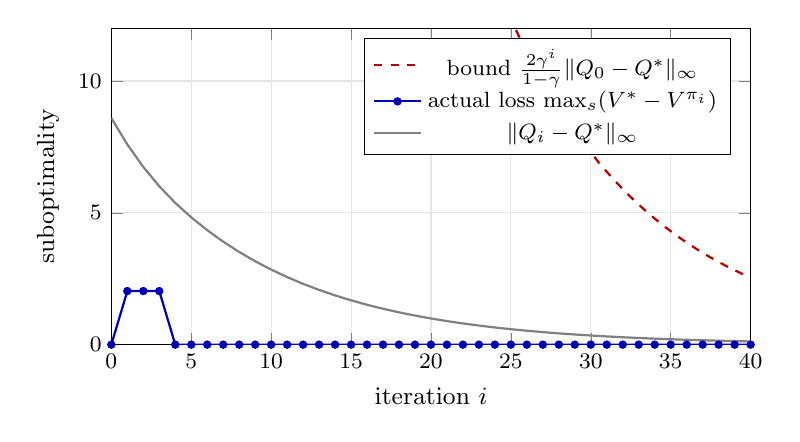
\begin{tikzpicture}
\begin{axis}[width=0.8\linewidth, height=5.6cm, xmin=0, xmax=40, ymin=0, ymax=12, xlabel={iteration $i$}, ylabel={suboptimality}, grid=both, grid style={gray!20}, legend pos=north east, clip=true]
\addplot[red!70!black, dashed, thick, domain=0:40, samples=81] {171.875*0.9^x};
\addplot[blue!70!black, thick, mark=*, mark size=1.1pt] coordinates {(0.000000,0.000000) (1.000000,2.031250) (2.000000,2.031250) (3.000000,2.031250) (4.000000,0.000000) (5.000000,0.000000) (6.000000,0.000000) (7.000000,0.000000) (8.000000,0.000000) (9.000000,0.000000) (10.000000,0.000000) (11.000000,0.000000) (12.000000,0.000000) (13.000000,0.000000) (14.000000,0.000000) (15.000000,0.000000) (16.000000,0.000000) (17.000000,0.000000) (18.000000,0.000000) (19.000000,0.000000) (20.000000,0.000000) (21.000000,0.000000) (22.000000,0.000000) (23.000000,0.000000) (24.000000,0.000000) (25.000000,0.000000) (26.000000,0.000000) (27.000000,0.000000) (28.000000,0.000000) (29.000000,0.000000) (30.000000,0.000000) (31.000000,0.000000) (32.000000,0.000000) (33.000000,0.000000) (34.000000,0.000000) (35.000000,0.000000) (36.000000,0.000000) (37.000000,0.000000) (38.000000,0.000000) (39.000000,0.000000) (40.000000,0.000000)};
\addplot[gray, thick] coordinates {(0.000000,8.593750) (1.000000,7.593750) (2.000000,6.738750) (3.000000,6.005700) (4.000000,5.375479) (5.000000,4.827257) (6.000000,4.340689) (7.000000,3.905237) (8.000000,3.514215) (9.000000,3.162614) (10.000000,2.846288) (11.000000,2.561636) (12.000000,2.305464) (13.000000,2.074915) (14.000000,1.867422) (15.000000,1.680680) (16.000000,1.512611) (17.000000,1.361350) (18.000000,1.225215) (19.000000,1.102694) (20.000000,0.992424) (21.000000,0.893182) (22.000000,0.803864) (23.000000,0.723477) (24.000000,0.651130) (25.000000,0.586017) (26.000000,0.527415) (27.000000,0.474673) (28.000000,0.427206) (29.000000,0.384486) (30.000000,0.346037) (31.000000,0.311433) (32.000000,0.280290) (33.000000,0.252261) (34.000000,0.227035) (35.000000,0.204331) (36.000000,0.183898) (37.000000,0.165508) (38.000000,0.148958) (39.000000,0.134062) (40.000000,0.120656)};
\legend{bound $\tfrac{2\gamma^i}{1-\gamma}\norm{Q_0-Q^*}$, actual loss $\max_s(V^*-V^{\pi_i})$, $\norm{Q_i-Q^*}$}
\end{axis}
\end{tikzpicture}
\caption{Guaranteed versus actual loss of the greedy policy (Example~\ref{ex:greedy}; original figure). The bound is vacuous (above the plotted range) until $i\approx26$, yet the greedy policy is already optimal from $i=4$. The theorem is a worst-case guarantee, not a prediction.}
\label{fig:greedy}
\end{figure}

%=====================================================================
\section{Number of Iterations of Value Iteration \slides{66--74}}\label{sec:iters}
%=====================================================================
\emph{Note: as with exact policy evaluation, the companion note lists this derivation as ``on the slides only''.}

If we want an $\epsilon$ error on the quality of the policy, we can determine the number of iterations $i$ by solving for it in
\[
\frac{2\gamma^i}{1-\gamma}\norm{Q_0-Q^*}\le\epsilon .
\]

\begin{proposition}[Number of iterations for an $\epsilon$-optimal greedy policy]\label{prop:iters}
Let $Q_0\in[0,1/(1-\gamma)]^{|\cS||\cA|}$ (e.g.\ $Q_0=0$) and rewards in $[0,1]$. If
\[
i\;\ge\;\frac{1}{1-\gamma}\,\ln\!\Big(\frac{2}{\epsilon(1-\gamma)^2}\Big),
\]
then $V^{\pi_i}(s)\ge V^*(s)-\epsilon$ for every state $s$.
\end{proposition}
\begin{proof}
\emph{Step 1 (slides 67--69).} $Q^*$ also lies in $[0,1/(1-\gamma)]$ (Fact~\ref{fact:range}), so by the infinity norm $\norm{Q_0-Q^*}\le1/(1-\gamma)$ (for $Q_0=0$ it is just $\norm{Q^*}\le1/(1-\gamma)$). Hence by Theorem~\ref{thm:greedy} it suffices that $\dfrac{2\gamma^i}{(1-\gamma)^2}\le\epsilon$.

\emph{Step 2 (slides 70--71).} Write $\gamma=1-(1-\gamma)$ (``add and subtract~1'') and use $1+x\le e^x$ for all real $x$ with $x=-(1-\gamma)$:
\[
\gamma^i=\big(1-(1-\gamma)\big)^i\le e^{-(1-\gamma)i}.
\]
So it suffices that $\dfrac{2e^{-(1-\gamma)i}}{(1-\gamma)^2}\le\epsilon$, i.e.\ $e^{-(1-\gamma)i}\le\dfrac{\epsilon(1-\gamma)^2}{2}$.

\emph{Step 3 (slides 72--74).} Take logarithms and use $\ln(1/x)=-\ln x$: $-(1-\gamma)i\le-\ln\!\big(\tfrac{2}{\epsilon(1-\gamma)^2}\big)$. Isolating $i$ gives the claimed condition.
\end{proof}

\begin{intuition}
\emph{Worked numbers} ($\epsilon=0.01$): for $\gamma=0.9$ the condition is $i\ge10\ln(20\,000)=99.03$, so \textbf{100 iterations}; for $\gamma=0.99$ it is $i\ge100\ln(2\cdot10^6)=1450.9$, so \textbf{1451 iterations}. Making $\gamma$ closer to one multiplies the work by about $10\times$ per extra ``nine'', while making $\epsilon$ ten times smaller adds only $\ln10/(1-\gamma)\approx23$ iterations at $\gamma=0.9$. In words: accuracy is cheap (logarithmic in $1/\epsilon$), the planning horizon $1/(1-\gamma)$ is what costs. Multiplying by the per-iteration cost, an $\epsilon$-optimal policy takes $O\big(|\cS|^2|\cA|\cdot\tfrac{1}{1-\gamma}\ln\tfrac1{\epsilon(1-\gamma)^2}\big)$ arithmetic operations. (Replacing $\ln(1/\gamma)$ by its lower bound $1-\gamma$ is a safe simplification: it can only make the required $i$ larger, e.g.\ $99.0$ instead of $94.0$ for $\gamma=0.9$.)
\end{intuition}

\begin{figure}[htbp]
\centering
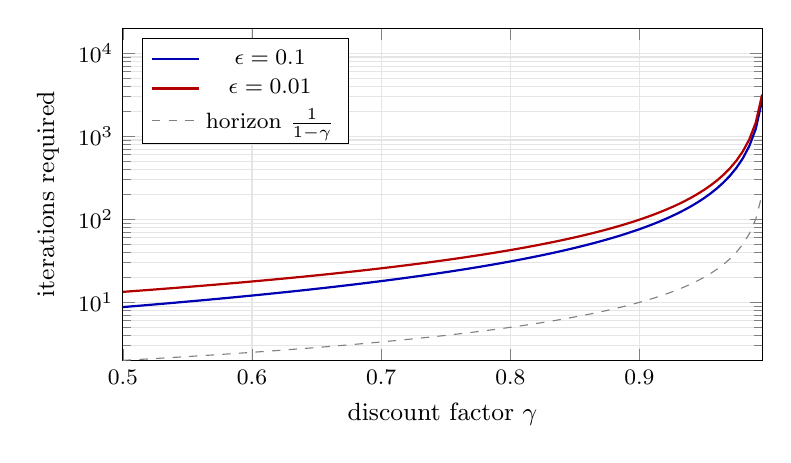
\begin{tikzpicture}
\begin{axis}[width=0.8\linewidth, height=5.8cm, xmin=0.5, xmax=0.995, ymode=log, ymin=2, ymax=20000, xlabel={discount factor $\gamma$}, ylabel={iterations required}, grid=both, grid style={gray!20}, legend pos=north west]
\addplot[blue!70!black, thick, domain=0.5:0.995, samples=100] {ln(2/(0.1*(1-x)^2))/(1-x)};
\addplot[red!70!black, thick, domain=0.5:0.995, samples=100] {ln(2/(0.01*(1-x)^2))/(1-x)};
\addplot[gray, dashed, domain=0.5:0.995, samples=100] {1/(1-x)};
\legend{$\epsilon=0.1$, $\epsilon=0.01$, horizon $\tfrac{1}{1-\gamma}$}
\end{axis}
\end{tikzpicture}
\caption{Iterations sufficient for an $\epsilon$-optimal greedy policy (Proposition~\ref{prop:iters}; original figure, slides 66--74 only give the formula). The curves track the horizon $1/(1-\gamma)$ up to a logarithmic factor.}
\label{fig:iters}
\end{figure}

%=====================================================================
\section{Another Note on Value Iteration \slide{75}}
%=====================================================================
$Q_t$ is approximating $Q^*$, and from $Q_t$ we compute a policy $\pi_t$. \emph{However}, $Q_t$ is generally different from $Q^{\pi_t}$ until we converge to (approximately) $Q^*$. For example, $Q_0$ is just a random initial guess, which may not correspond to any policy's Q-value.

\begin{figure}[htbp]
\centering
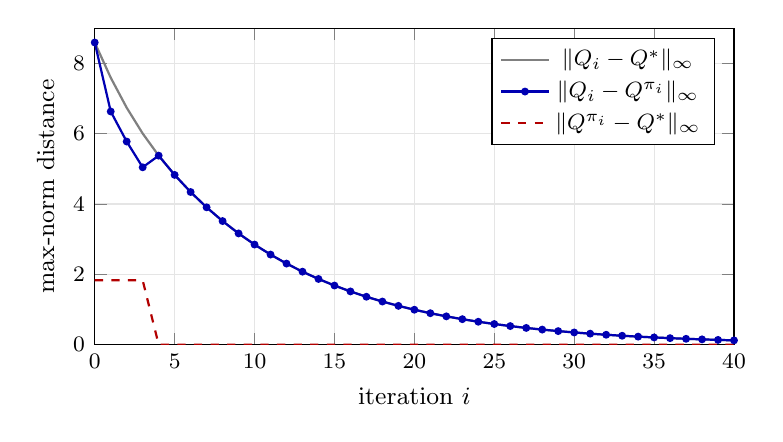
\begin{tikzpicture}
\begin{axis}[width=0.8\linewidth, height=5.6cm, xmin=0, xmax=40, ymin=0, ymax=9, xlabel={iteration $i$}, ylabel={max-norm distance}, grid=both, grid style={gray!20}, legend pos=north east]
\addplot[gray, thick] coordinates {(0.000000,8.593750) (1.000000,7.593750) (2.000000,6.738750) (3.000000,6.005700) (4.000000,5.375479) (5.000000,4.827257) (6.000000,4.340689) (7.000000,3.905237) (8.000000,3.514215) (9.000000,3.162614) (10.000000,2.846288) (11.000000,2.561636) (12.000000,2.305464) (13.000000,2.074915) (14.000000,1.867422) (15.000000,1.680680) (16.000000,1.512611) (17.000000,1.361350) (18.000000,1.225215) (19.000000,1.102694) (20.000000,0.992424) (21.000000,0.893182) (22.000000,0.803864) (23.000000,0.723477) (24.000000,0.651130) (25.000000,0.586017) (26.000000,0.527415) (27.000000,0.474673) (28.000000,0.427206) (29.000000,0.384486) (30.000000,0.346037) (31.000000,0.311433) (32.000000,0.280290) (33.000000,0.252261) (34.000000,0.227035) (35.000000,0.204331) (36.000000,0.183898) (37.000000,0.165508) (38.000000,0.148958) (39.000000,0.134062) (40.000000,0.120656)};
\addplot[blue!70!black, thick, mark=*, mark size=1pt] coordinates {(0.000000,8.593750) (1.000000,6.631579) (2.000000,5.776579) (3.000000,5.043529) (4.000000,5.375479) (5.000000,4.827257) (6.000000,4.340689) (7.000000,3.905237) (8.000000,3.514215) (9.000000,3.162614) (10.000000,2.846288) (11.000000,2.561636) (12.000000,2.305464) (13.000000,2.074915) (14.000000,1.867422) (15.000000,1.680680) (16.000000,1.512611) (17.000000,1.361350) (18.000000,1.225215) (19.000000,1.102694) (20.000000,0.992424) (21.000000,0.893182) (22.000000,0.803864) (23.000000,0.723477) (24.000000,0.651130) (25.000000,0.586017) (26.000000,0.527415) (27.000000,0.474673) (28.000000,0.427206) (29.000000,0.384486) (30.000000,0.346037) (31.000000,0.311433) (32.000000,0.280290) (33.000000,0.252261) (34.000000,0.227035) (35.000000,0.204331) (36.000000,0.183898) (37.000000,0.165508) (38.000000,0.148958) (39.000000,0.134062) (40.000000,0.120656)};
\addplot[red!70!black, thick, dashed] coordinates {(0,1.828125) (1,1.828125) (2,1.828125) (3,1.828125) (4,0.000000) (5,0.000000) (6,0.000000) (7,0.000000) (8,0.000000) (9,0.000000) (10,0.000000) (11,0.000000) (12,0.000000) (13,0.000000) (14,0.000000) (15,0.000000) (16,0.000000) (17,0.000000) (18,0.000000) (19,0.000000) (20,0.000000) (21,0.000000) (22,0.000000) (23,0.000000) (24,0.000000) (25,0.000000) (26,0.000000) (27,0.000000) (28,0.000000) (29,0.000000) (30,0.000000) (31,0.000000) (32,0.000000) (33,0.000000) (34,0.000000) (35,0.000000) (36,0.000000) (37,0.000000) (38,0.000000) (39,0.000000) (40,0.000000)};
\legend{$\norm{Q_i-Q^*}$, $\norm{Q_i-Q^{\pi_i}}$, $\norm{Q^{\pi_i}-Q^*}$}
\end{axis}
\end{tikzpicture}
\caption{On Example~\ref{ex:toy}: the iterate $Q_i$ is far from the Q-function $Q^{\pi_i}$ of its own greedy policy for many iterations, even after $\pi_i$ has become optimal ($i\ge4$, where $\norm{Q^{\pi_i}-Q^*}=0$). Ties at $i=0$ are broken towards $a$. (Original figure; slide 75 is text only.)}
\label{fig:qpi}
\end{figure}

\begin{intuition}
Value iteration is \emph{not} ``evaluate a policy, then improve it''. The intermediate tables $Q_i$ are only approximations of $Q^*$; there may not exist any policy whose Q-function equals $Q_i$. In the two-state MDP, $Q_1=r$, but every policy has strictly positive values, so $Q^\pi(s,a)=r(s,a)+\gamma\E V^\pi(s')>r(s,a)$ for all $\pi$: $Q_1$ is the Q-function of \emph{no} policy. Only in the limit does $Q_i$ become $Q^*=Q^{\pi^*}$. This is why Theorem~\ref{thm:greedy} is needed at all: it tells us what the greedy policy of an imperfect $Q_i$ is worth.
\end{intuition}
%=====================================================================
\section{Summary}
%=====================================================================
\subsection{Comparison of the methods and results}
\begin{center}
\small
\renewcommand{\arraystretch}{1.25}
\begin{tabular}{@{}>{\raggedright\arraybackslash}p{2.5cm}>{\raggedright\arraybackslash}p{2.9cm}>{\raggedright\arraybackslash}p{3.7cm}>{\raggedright\arraybackslash}p{4.9cm}c@{}}
\toprule
\textbf{Method} & \textbf{Computes / operator} & \textbf{Cost} & \textbf{Guarantee} & \textbf{Slides}\\
\midrule
Exact policy evaluation & $V^\pi$; solve $(I-\gamma P^\pi)V=r^\pi$ & $O(|\cS|^3)$ & exact (Prop.~\ref{prop:exact}) & 16--22\\
Iterative policy evaluation & $V^\pi$; $\Bpi$ (affine, $\gamma$-contraction) & $O(|\cS|^2)$ per sweep; $O(|\cS|^2\ln\frac1\epsilon)$ in total & $\norm{V_i-V^\pi}\le\gamma^i\norm{V_0-V^\pi}$ (Cor.~\ref{cor:pe}) & 29--38\\
Naive policy search & $\pi^*$; evaluate every policy & $O(|\cA|^{|\cS|}|\cS|^3)$ & exact, but exponential & 39--42\\
Value iteration & $Q^*$; $\Bell$ (non-linear, $\gamma$-contraction) & $O(|\cS|^2|\cA|)$ per iteration & $\norm{Q_i-Q^*}\le\gamma^i\norm{Q_0-Q^*}$ (Thm.~\ref{thm:vi}) & 49--53\\
Greedy policy from VI & $\pi_i=\argmax_aQ_i$ & free (an $\argmax$) & $V^{\pi_i}\ge V^*-\frac{2\gamma^i}{1-\gamma}\norm{Q_0-Q^*}$ (Thm.~\ref{thm:greedy}) & 54--65\\
$\epsilon$-optimal policy & number of iterations & $i\ge\frac1{1-\gamma}\ln\frac{2}{\epsilon(1-\gamma)^2}$ & $V^{\pi_i}\ge V^*-\epsilon$ (Prop.~\ref{prop:iters}) & 66--74\\
\bottomrule
\end{tabular}
\end{center}

\subsection{Cost scaling}
\begin{figure}[htbp]
\centering
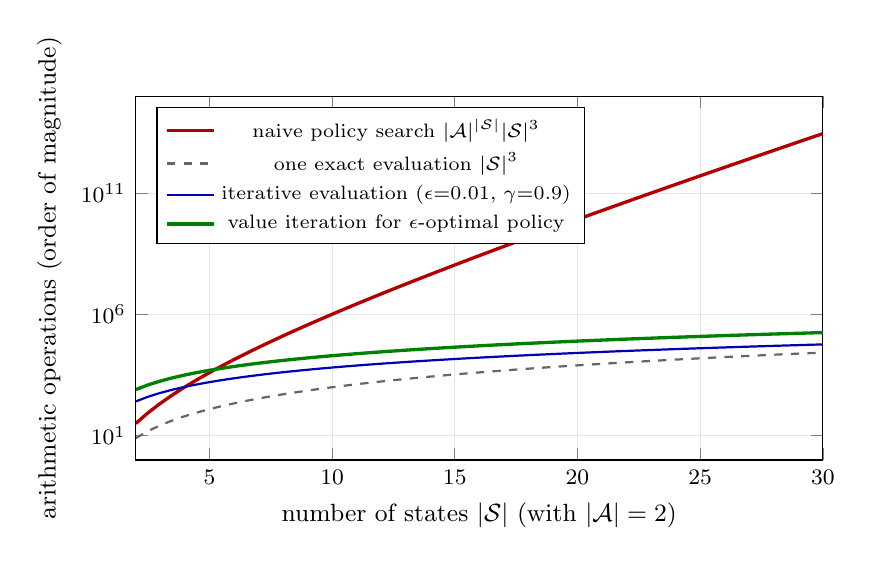
\begin{tikzpicture}
\begin{axis}[width=0.85\linewidth, height=6.2cm, xmin=2, xmax=30, ymode=log, ymin=1, ymax=1e15, xlabel={number of states $|\cS|$ (with $|\cA|=2$)}, ylabel={arithmetic operations (order of magnitude)}, grid=both, grid style={gray!20}, legend style={at={(0.03,0.97)}, anchor=north west, font=\scriptsize}]
\addplot[red!70!black, very thick, domain=2:30, samples=60] {2^x*x^3};
\addplot[black!60, thick, dashed, domain=2:30, samples=60] {x^3};
\addplot[blue!70!black, thick, domain=2:30, samples=60] {65*x^2};
\addplot[green!50!black, very thick, domain=2:30, samples=60] {200*x^2};
\legend{{naive policy search $|\cA|^{|\cS|}|\cS|^3$},{one exact evaluation $|\cS|^3$},{iterative evaluation ($\epsilon{=}0.01$, $\gamma{=}0.9$)},{value iteration for $\epsilon$-optimal policy}}
\end{axis}
\end{tikzpicture}
\caption{Qualitative cost comparison (original figure; constants dropped, iteration counts from the worked examples: $65$ sweeps for evaluation, $100$ iterations $\times\,|\cA|=2$ for value iteration, $\gamma=0.9$, $\epsilon=0.01$). Enumerating policies explodes exponentially; value iteration stays polynomial.}
\label{fig:costs}
\end{figure}

\subsection{Key take-aways}
\begin{itemize}
  \item \textbf{Policy evaluation is a linear problem.} $V^\pi=(I-\gamma P^\pi)^{-1}r^\pi$ exactly in $O(|\cS|^3)$, or approximately by iterating $V_{i+1}=r^\pi+\gamma P^\pi V_i$ at $O(|\cS|^2)$ per sweep and $O(\ln\frac1\epsilon)$ sweeps.
  \item \textbf{Contractions are the engine.} A $k$-contraction on a complete metric space has a unique fixed point and fixed-point iteration converges to it at rate $k^i$ (Banach). Both $\Bpi$ and $\Bell$ are $\gamma$-contractions in the sup-norm, because rewards cancel and averages cannot exceed maxima; hence $V^\pi$, $V^*$ and $Q^*$ are their unique fixed points.
  \item \textbf{Value iteration} $Q_{i+1}=\Bell Q_i$ converges geometrically, $\norm{Q_i-Q^*}\le\gamma^i\norm{Q_0-Q^*}$, at $O(|\cS|^2|\cA|)$ per iteration, avoiding the $|\cA|^{|\cS|}$ policy enumeration.
  \item \textbf{The greedy policy is near-optimal, with a $\frac{2}{1-\gamma}$ penalty:} $V^{\pi_i}\ge V^*-\frac{2\gamma^i}{1-\gamma}\norm{Q_0-Q^*}$, so $i\ge\frac1{1-\gamma}\ln\frac2{\epsilon(1-\gamma)^2}$ iterations give an $\epsilon$-optimal policy: accuracy is logarithmic, the horizon $\frac1{1-\gamma}$ is what costs.
  \item \textbf{The intermediate $Q_i$ are not policy values.} Value iteration does not alternate evaluation and improvement; $Q_i$ is generally different from $Q^{\pi_i}$ until convergence, and the bound in Theorem~\ref{thm:greedy} is a worst-case guarantee that is often very pessimistic (\figref{fig:greedy}).
\end{itemize}

%=====================================================================
\appendix
\section{Supplementary: Banach's Theorem, Existence and Rate}\label{app:banach}
%=====================================================================
\emph{This appendix is \textbf{not covered on the slides}; it comes from the companion note only. The slides state the uniqueness half of Theorem~\ref{thm:banach} (slide 25) and then use convergence of fixed-point iteration (slides 23--24, 29--38, 49--53) without proving it.}

\begin{proof}[Proof of Theorem~\ref{thm:banach}: existence and rate]
\emph{Existence.} From $x_{i+1}=f(x_i)$ we get $d(x_{i+1},x_i)=d(f(x_i),f(x_{i-1}))\le k\,d(x_i,x_{i-1})$, hence $d(x_{i+1},x_i)\le k^i\,d(x_1,x_0)$ by induction. For $j>i$ the triangle inequality gives
\[
d(x_j,x_i)\le\sum_{l=i}^{j-1}d(x_{l+1},x_l)\le\sum_{l=i}^{j-1}k^l\,d(x_1,x_0)\le\frac{k^i}{1-k}\,d(x_1,x_0),
\]
which tends to $0$ as $i\to\infty$: the sequence is Cauchy, and by completeness it has a limit $x^*$. A contraction is continuous (it is Lipschitz), so $f(x^*)=f(\lim x_i)=\lim f(x_i)=\lim x_{i+1}=x^*$.

\emph{Rate.} Since $f(x^*)=x^*$, $d(x_i,x^*)=d(f(x_{i-1}),f(x^*))\le k\,d(x_{i-1},x^*)$, and induction gives $d(x_i,x^*)\le k^i\,d(x_0,x^*)$.
\end{proof}

\begin{intuition}
The sequence of iterates is a walk whose steps shrink geometrically ($d(x_{i+1},x_i)\le k^id(x_1,x_0)$), so the \emph{total remaining path length} is a convergent geometric series. A walk with summable steps cannot wander forever: it settles somewhere (completeness says that ``somewhere'' is a point of the space), and by continuity that limit must be unmoved by $f$. The rate is then just the contraction inequality applied to the pair $(x_{i-1},x^*)$.
\end{intuition}

%=====================================================================
\section{Supplementary: Self-Check List from the Companion Note}\label{app:selfcheck}
%=====================================================================
\emph{Study aid reproduced from the companion note (not a slide topic). ``State'' means: write the statement with assumptions and say in one sentence what it claims (for an algorithm: write its steps). ``Prove'' means: write the proof without looking. The last column gives the proof video of the same lecture on Classroom and where the item lives in these notes.}

\begin{center}
\small
\renewcommand{\arraystretch}{1.2}
\begin{tabular}{@{}>{\raggedright\arraybackslash}p{6.0cm}cc>{\raggedright\arraybackslash}p{4.9cm}@{}}
\toprule
\textbf{Item} & \textbf{state} & \textbf{prove} & \textbf{Video / location here}\\
\midrule
On the slides only: exact policy evaluation (slides 16--22) & $\square$ & $\square$ & Prop.~\ref{prop:exact}, \S\ref{sec:exact}\\
Definition 1 (contraction) & $\square$ & & \S\ref{sec:contr}\\
Theorem 2 (Banach) & $\square$ & $\square$ & \texttt{ch05-banach.mp4}; \S\ref{sec:contr}, App.~\ref{app:banach}\\
Definition 3 (Bellman operators) & $\square$ & & \S\ref{sec:itpe}\\
Theorem 4 (both $\gamma$-contractions) & $\square$ & $\square$ & \texttt{ch05-contraction.mp4}; \S\ref{sec:thm4}, \S\ref{sec:optcontr}\\
Corollary 5 (what the fixed points are) & $\square$ & $\square$ & \texttt{ch05-vi.mp4}; \S\ref{sec:vi}\\
Algorithm A (iterative policy evaluation) & $\square$ & & \S\ref{sec:itpe}\\
Corollary 6 (convergence and cost) & $\square$ & $\square$ & \texttt{ch05-vi.mp4}; \S\ref{sec:peiters}\\
Algorithm B (value iteration) & $\square$ & & \S\ref{sec:vi}\\
Theorem 7 (VI converges geometrically) & $\square$ & $\square$ & \texttt{ch05-vi.mp4}; \S\ref{sec:vi}\\
Theorem 8 (quality of the greedy policy) & $\square$ & $\square$ & \texttt{ch05-greedyquality.mp4}; \S\ref{sec:greedy}\\
On the slides only: iterations of VI for an $\epsilon$-optimal policy (slides 66--74) & $\square$ & $\square$ & Prop.~\ref{prop:iters}, \S\ref{sec:iters}\\
\bottomrule
\end{tabular}
\end{center}

\end{document}
